\chapter{Diseño e Implementación} % Main chapter title
\label{Chapter3} 

En este capítulo se presentan y fundamentan las decisiones adoptadas durante el diseño del equipo, la implementación de la placa electrónica y el desarrollo del firmware.

\section{Diseño del hardware}
\label{sec:hardware}

Un aspecto muy importante que se tuvo en cuenta desde el momento mismo de seleccionar los componentes que se utilizaron en el diseño del equipo es la realidad del medio en el que fabricará y comercializará el producto. EQUISER es una microempresa que comercializa actualmente, en promedio, dos unidades al mes. Esto determina que la fabricación se efectúe en lotes de entre diez y veinte unidades, que representan cantidades muy pequeñas para el estándar de la industria electrónica. Si bien la firma tiene capacidad para importar componentes del exterior, los constantes cambios en las políticas aduaneras del país y la incidencia del costo de los fletes en compras pequeñas llevaron a  minimizar la dependencia de proveedores extranjeros.

En este contexto, y como una solución de compromiso entre la disponibilidad local, la facilidad de montaje, el costo y las prestaciones, se adoptó como procesador principal del equipo el módulo ESP-WROOM-32D de la empresa Espressif. Basado en un procesador de doble núcleo Xtensa de 32bits, que puede operar con una frecuencia de hasta 240 MHz, este microcontrolador dispone de 520 kB de memoria RAM interna y se integra en el módulo 4 MB de memoria flash. Implementa entradas y salidas tanto digitales como analógicas, y puertos de comunicaciones con los protocolos SPI, I2C y UART. Para la comunicación inalámbrica están disponibles una interfaz Bluetooth que puede funcionar con las versiones 2 y 4 del protocolo, y una interfaz WiFi que opera en 2.4 GHz que cumple con las variantes b, g y n del estándar IEEE802.11.

Este módulo se presenta como el sucesor del ESP8266, un diseño pensado originalmente como interfaz WiFi de bajo costo para pequeños microcontroladores, que ganó una cuota importante del mercado cuando el fabricante puso a disposición del público las herramientas para desarrollar versiones propias del firmware. Esto permitió integrar la aplicación directamente dentro del módulo y convertirlo de esta forma en el procesador principal del sistema. Uno de los factores clave del éxito de esta propuesta es el costo y la relativa facilidad de montaje del módulo, características que se mantienen en el ESP-WROM-32D, la versión seleccionada para este diseño. 

En la figura \ref{fig:DiagramaBloques} se presenta el diagrama de bloques del nuevo equipo. Si se lo compara con el de la figura \ref{fig:BloquesActual}, que corresponde al diseño original del equipo, podemos observar las siguientes diferencias:

\begin{figure}[ht]
	\centering
	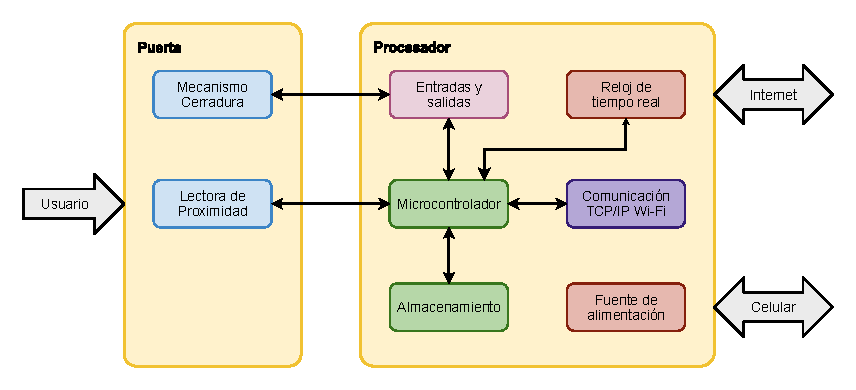
\includegraphics[width=\textwidth]{Figures/BloquesNuevo.pdf}
	\caption{Diagrama de bloques del equipo desarrollado}
	\label{fig:DiagramaBloques}
\end{figure}

\begin{itemize}
	\item Se unificaron las dos unidades funcionales del equipo anterior en el procesador. Así, quedó instalada en la puerta únicamente la placa electrónica que implementa la antena de RFID con el circuito integrado responsable de la generación del campo electromagnético y el procesamiento analógico de la señal recibida. Esto permite además de reducir la cantidad de componentes y centralizar en el firmware principal todo el procesamiento de la comunicación con la tarjeta de proximidad.
	\item En el bloque de entradas y salidas se cambió la conexión con el sistema de cerradura para  controlar indistintamente sistemas electromagnéticos o motorizados. Asimismo se agregaron sensores de fin de carrera para el mecanismo de la cerradura, lo que además de aumentar la confiabilidad del sistema permite prolongar la vida útil de los componentes al evitar esfuerzos innecesarios.
	\item Se cambió el bloque de comunicaciones Bluetooth por una interfaz WiFi, lo que permitió además adoptar el protocolo TPC/IP para la comunicación con el equipo. Esta interfaz puede operar en modo punto de acceso, lo que permite efectuar una comunicación punto a punto con el celular de la misma forma que se hacía con el Bluetooth. Pero también puede operar en modo estación, de esta forma el equipo puede conectarse una red WiFi existente y permitir la gestión desde cualquier dispositivo autorizado que tenga conexión con esta red.
	\item Se incorpora un reloj de tiempo real independiente del procesador que será el responsable de mantener la fecha y hora del sistema. Este bloque incluye una batería de respaldo que le permite continuar funcionando cuando el equipo no cuenta con alimentación.
\end{itemize}

\section{Prototipo del hardware}
\label{sec:prototipo}

En el diseño de la placa electrónica se siguieron los mismos criterios que ya se mencionaron en la sección \ref{sec:hardware} para la selección de los componentes. Se decidió mantener el gabinete actual, lo que determinó la geometría de la placa y la posición de la mayoría de los conectores. Se decidió también que la placa se realizaría con las capacidades de fabricación del único fabricante de circuitos impresos de la provincia, a quien se le encomendaría la producción del primer prototipo. Con estas restricciones el circuito impreso debía resolverse en dos capas y en un área de 87 x 66 mm. 

El trazado de las pistas de cobre no resultó simple, ya que como puede observarse en la figura \ref{fig:Componentes} una parte importante del área de la placa se encuentra ocupada por componentes, lo que sumado a la restricción de utilizar pistas de 0,5 mm y vías de 1 mm impuesta por el proceso de fabricación aumentó la dificultad del proceso de diseño. 

\begin{figure}[ht]
	\centering
	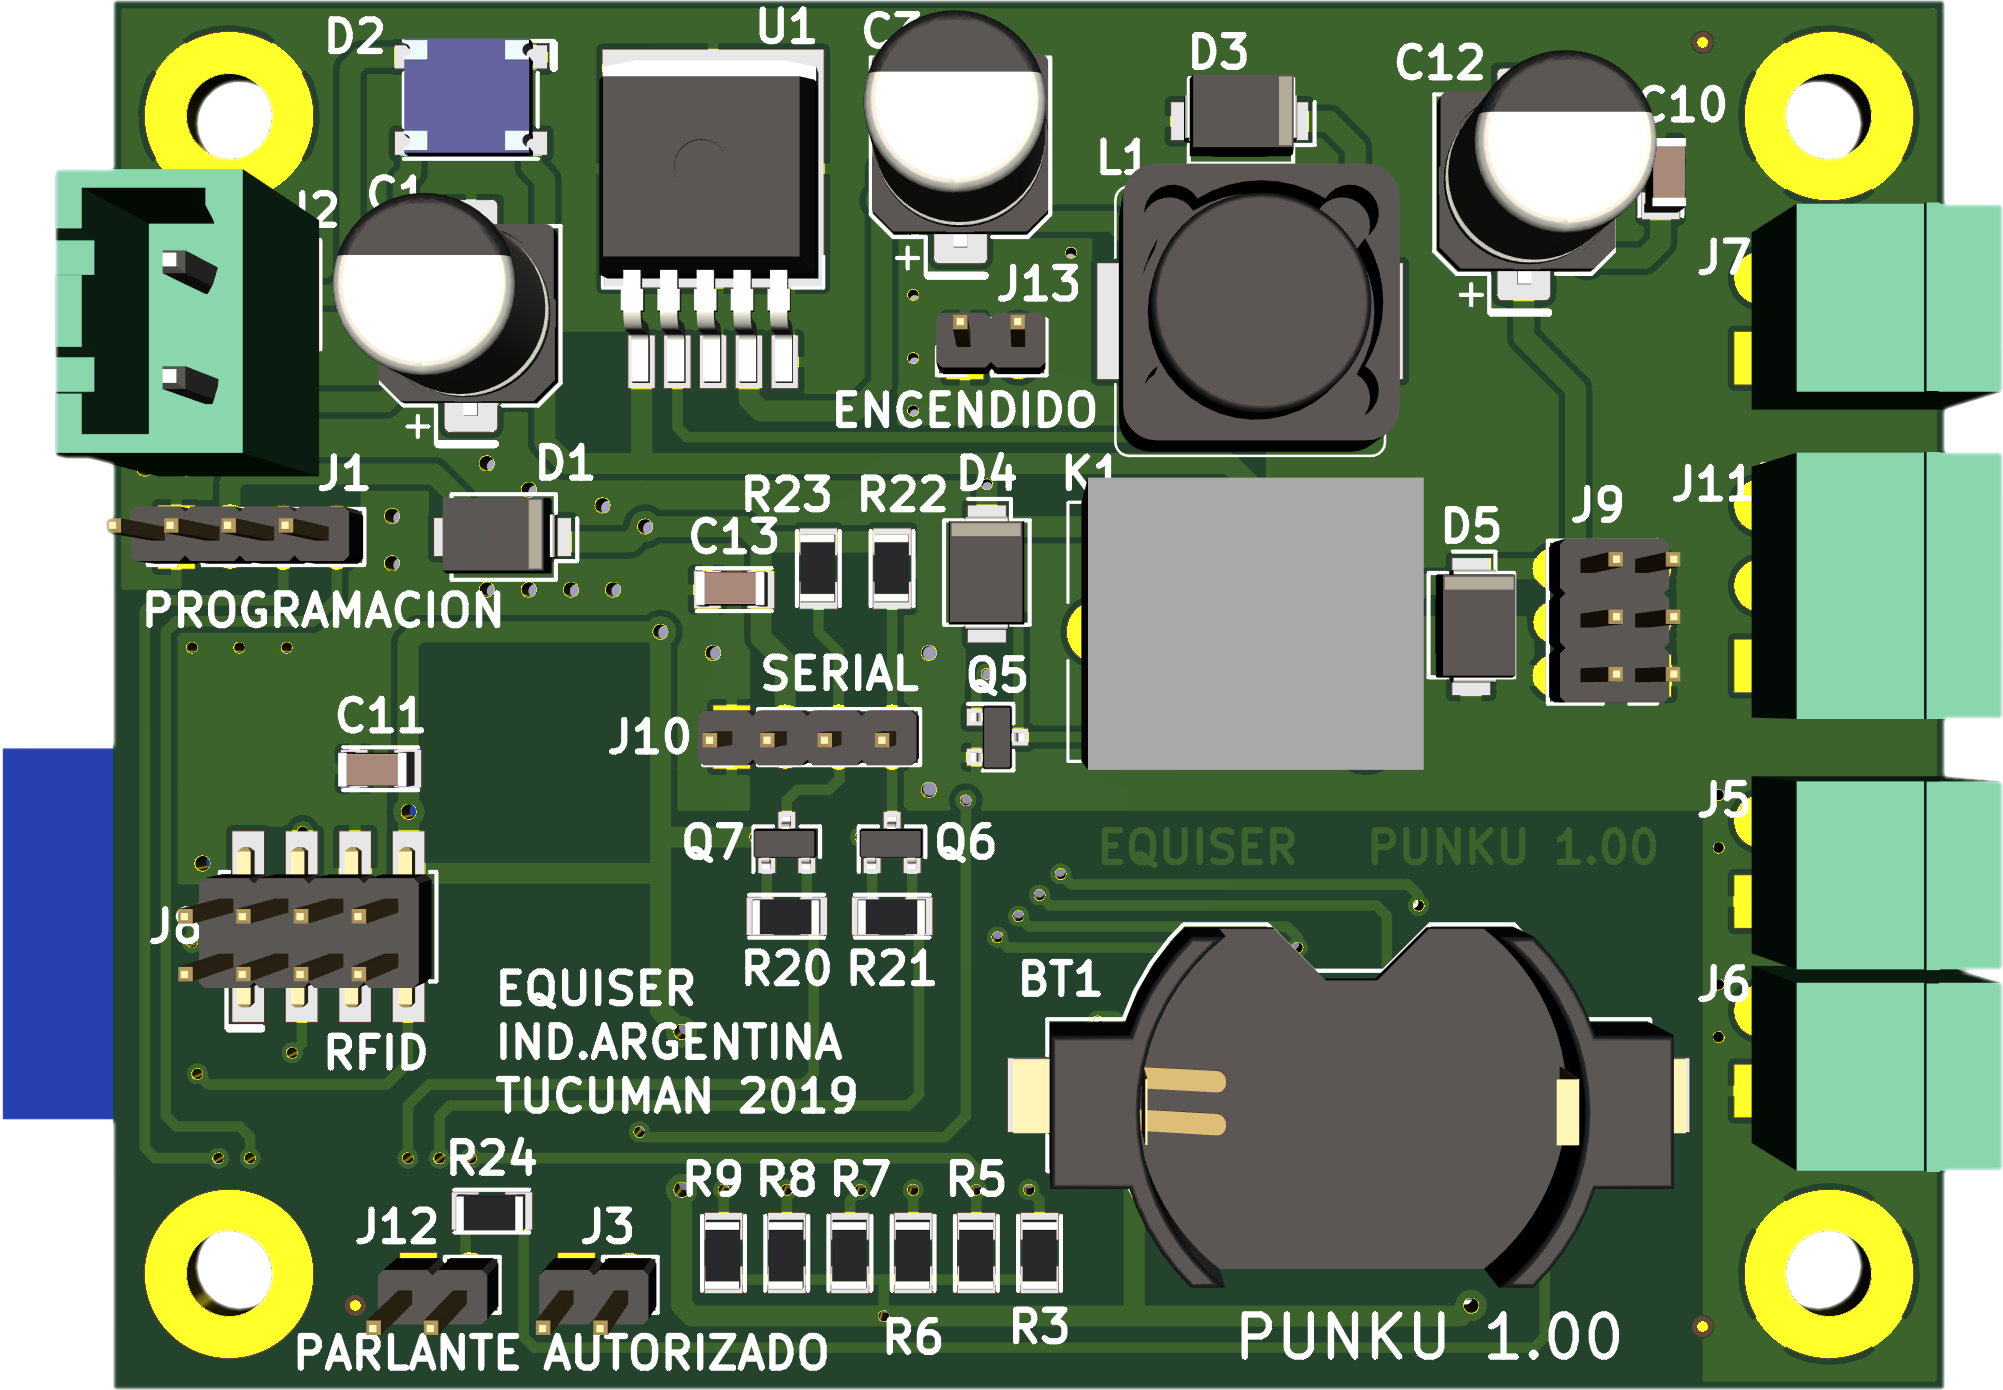
\includegraphics[width=0.9\textwidth]{Figures/ModeloPlaca.png}
	\caption[Modelo tridimensional de la placa electrónica]{Modelo tridimensional de la placa electrónica.}
	\label{fig:Componentes}
\end{figure}

Se efectuó un proceso de doble revisión sobre el diagrama esquemático del circuito y el diseño de la placa, y se incorporó una serie de recomendaciones efectuadas por los revisores como la utilización de los planos de tierra en las zonas de la placa generadoras de ruido electromagnético. Además de los controles mencionados, fue necesario un tercera revisión para detectar y corregir los últimos errores antes de la fabricación de la placa.

La construcción del prototipo se efectuó en forma manual, y durante el proceso se detectaron dificultades para el montaje en algunos componentes, originados en la separación entre los planos de masa y las pistas de señales. En el diseño se adoptó un valor similar al de separación entre pistas, pero debido a la falta de precisión en la máscara antisoldante que puede observarse en la imagen \ref{fig:ProblemasMascara}, este valor resultó pequeño. Durante el proceso de soldadura se generaron puentes de estaño entre los terminales de los componentes y el plano de masa circundante.

\begin{figure}[ht]
	\centering
	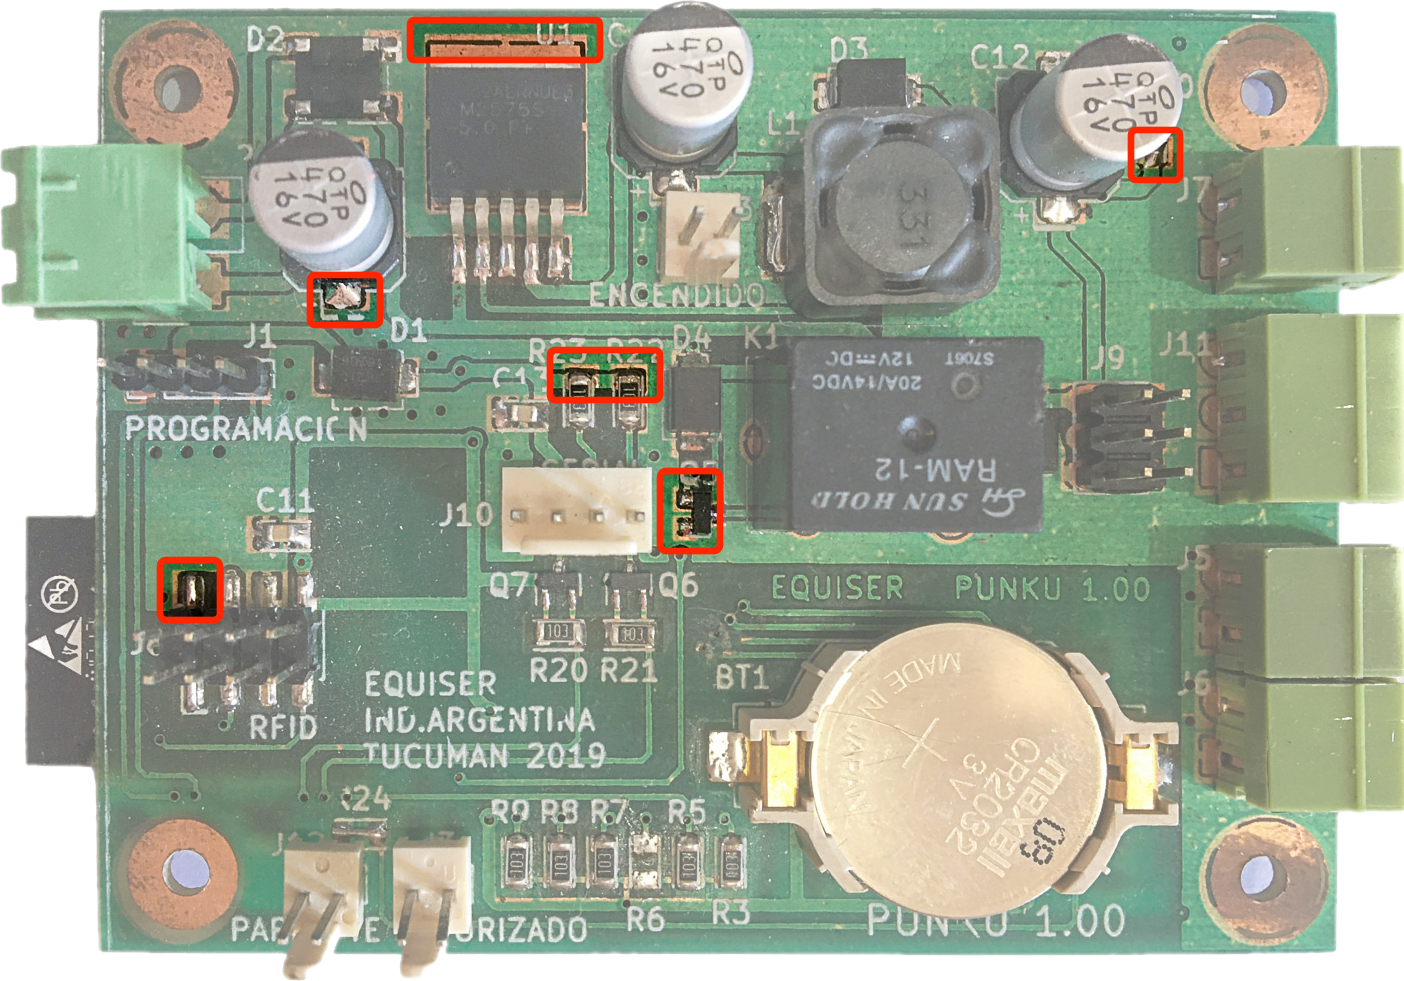
\includegraphics[width=0.9\textwidth]{Figures/LadoComponentes.png}
	\caption[Problemas con la  máscara antisoldante del prototipo]{Imagen que muestra la falta de precisión en la aplicación de la máscara antisoldante del prototipo.}
	\label{fig:ProblemasMascara}
\end{figure}

Para resolver este problema se removieron varios componentes del prototipo, y se recurrió al uso de abundantes cantidades \emph{flux} para volver a soldarlos evitando los cortocircuitos. Este proceso demandó mucho más tiempo de montaje, por lo que también se corrigió el diseño de la placa para aumentar el valor de guarda en los planos de masa, y evitar este problema en las siguientes placas. \todo{revisar}

\section{Diseño del firmware}
\label{sec:firmware}

\subsection{Arquitectura del firmware}
\label{sub:Arquitectura}

Uno de los objetivos planteados para el trabajo en la sección \ref{sec:objetivos} fue la reingeniería completa del firmware del equipo, que permitiera incorporar el uso de un sistema operativo de tiempo real y el reuso de los componentes comunes en otros proyectos similares. Para esto se decidió utilizar una arquitectura de capas, que se puede observar en el diagrama de componentes de la figura \ref{fig:DiagramaComponentes}. En la misma se pueden identificar claramente cuatro capas:

\begin{itemize}
	\item ESP-IDF: corresponde al conjunto de funciones provistas por el fabricante para facilitar el desarrollo en la plataforma. Allí se incluyen los controladores para los puertos GPIO, SPI, I2C y PWM. También se incluye la implementación del sistema de archivos FAT para tarjetas SD y de un servidor HTTP completo.

	\item Plataforma: implementa una capa de abstracción del hardware, también conocida como HAL (\emph{Hardware Abstraction Layer}), que permite independizar el resto del código desarrollado de la plataforma provista por el fabricante. Esta capa facilita la reutilización del resto de los componentes en proyectos similares y la eventual migración del firmware a otra plataforma.

	\item Controladores: implementa una serie de clases que se pueden reutilizar en otros proyectos fácilmente ya que no dependen del hardware ni de la aplicación.

	\item Aplicación: implementa la lógica propia del equipo mediante un conjunto de tareas que ejecutan concurrentemente en un sistema operativo de tiempo real.
\end{itemize}


\begin{figure}[ht]
	\centering
	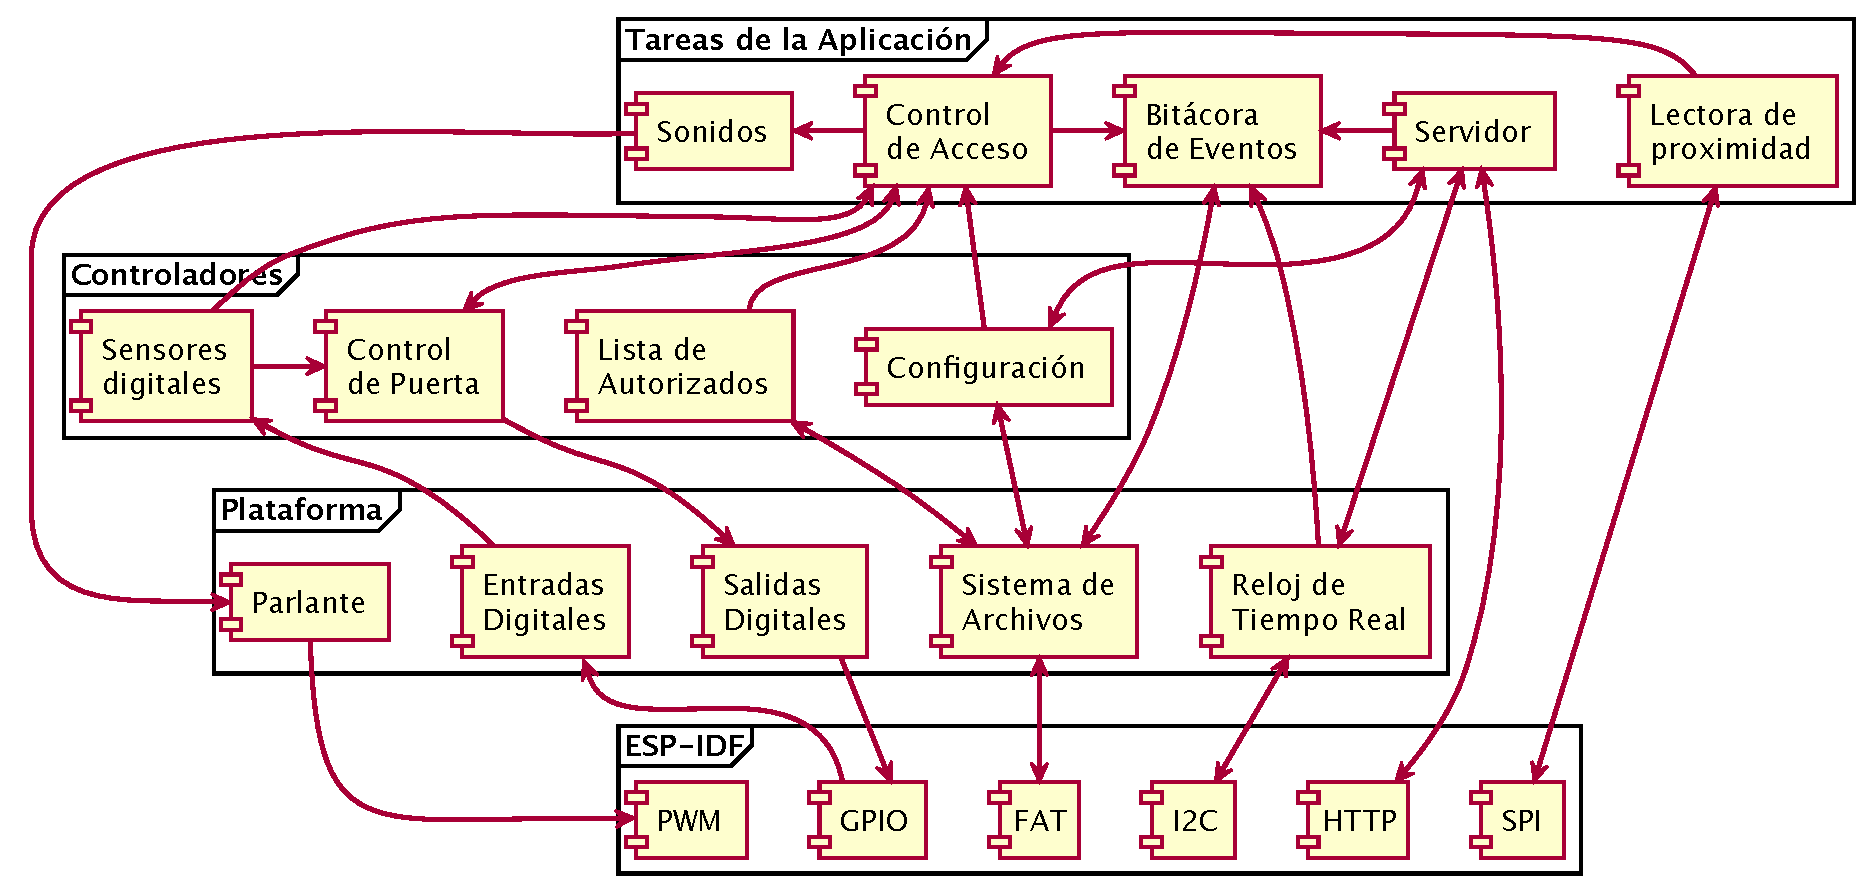
\includegraphics[width=\textwidth]{./Figures/PNK-DC001.pdf}
	\caption[Diagrama de componentes del firmware del equipo]{Diagrama de componentes del firmware del equipo.}
	\label{fig:DiagramaComponentes}
\end{figure}

Para el modelado de los componentes se utilizó el análisis orientado a objetos, lo que arrojó como resultado una colección de clases con sus respectivos métodos y atributos. Una imagen completa de este diseño se puede observar en el diagrama de clases que se muestra en la figura \ref{fig:DiagramaClases}. Allí solo están incluidos los componentes de las tres clases superiores desarrolladas en el marco del trabajo. En las siguientes subsecciones se explican brevemente las responsabilidades asignadas a cada una de estas clases.

\begin{figure}[H]
	\centering
	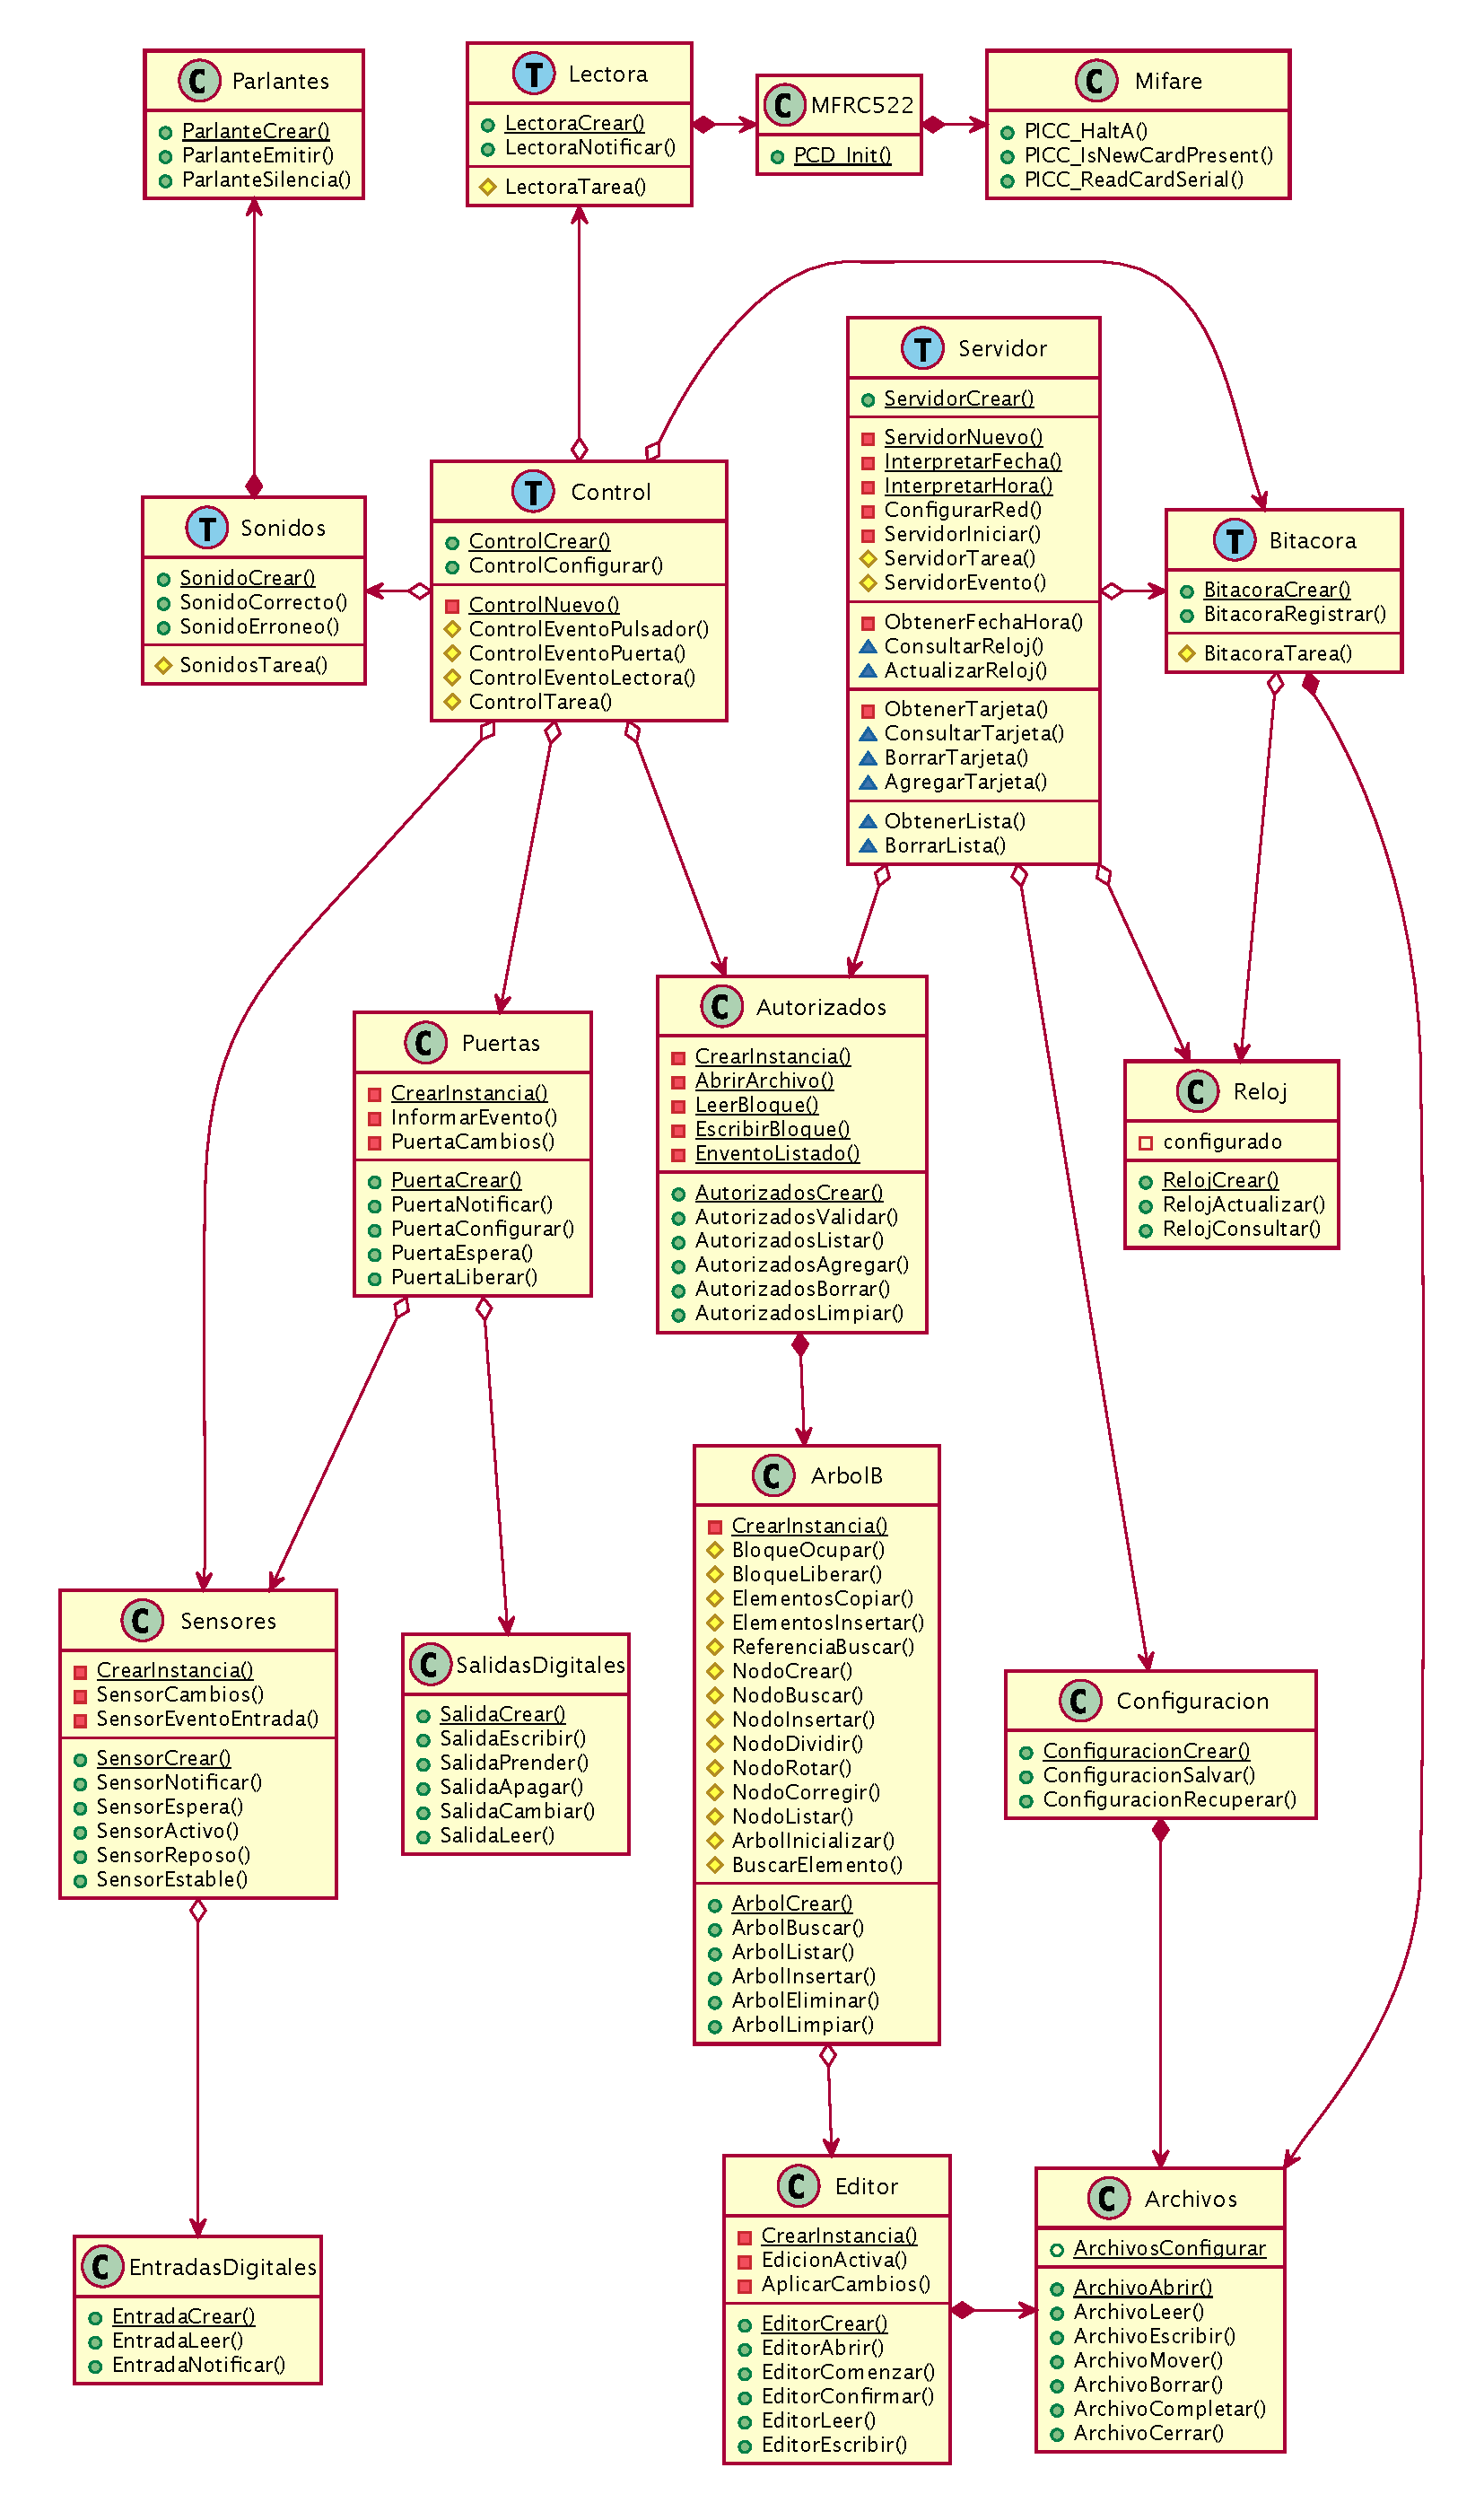
\includegraphics[width=\textwidth]{./Figures/PNK-DC002.pdf}
	\caption[Diagrama de clases del firmware del equipo]{Diagrama de clases del firmware del equipo.}
	\label{fig:DiagramaClases}
\end{figure}

\subsection{Capa de abstracción del hardware}

Esta capa contiene una colección de clases que encapsulan las funcionalidades del entorno de desarrollo provisto por el fabricante. Su principal objetivo es brindar una plataforma uniforme en comportamiento y documentación para el resto del firmware. Las clases que pertenecen a esta capa son:

\begin{itemize}
	\item EntradasDigitales: encapsula toda la gestión de un terminal digital utilizado como entrada. Permite configurarlo durante la creación del objeto, recuperar el estado actual y solicitar el envío de eventos generados por interrupciones disparadas por cambios en su estado.
	
	\item SalidasDigitales: encapsula toda la gestión de un terminal digital utilizado como salida. Permite configurarlo durante la creación del objeto, recuperar el estado actual y cambiarle el estado.
	
	\item Archivos: encapsula toda la gestión de un archivo almacenado en la tarjeta microSD del equipo. Después de la configuración de la propia clases permite la creación y el borrado de archivos, como así también la escritura y lectura de datos en ellos.
	
	\item Reloj: encapsula toda la gestión del reloj de tiempo real. Permite ajustar y recuperar la fecha y hora actuales.
	
	\item Parlantes: encapsula la gestión de un parlante conectado a un terminal digital que opera con modulación de ancho de pulso, o PWM (\emph{Pulse Width Modulation}). Permite, mediante la generación de una señal cuadrada de frecuencia arbitraria, emitir un tono en el parlante o silenciarlo.
\end{itemize}

\subsection{Capa de controladores}

Las clases que componen esta capa son independientes de la plataforma y de la aplicación, y por lo tanto son fácilmente reutilizables en otros proyectos. Para lograr este objetivo, la mayoría de ellas no utilizan  los servicios del sistema operativo, e implementan mecanismos de eventos para  extraer el código dependiente de la aplicación en otro componente. Las clases que pertenecen a esta capa son:

\begin{itemize}
	\item Puertas: encapsula toda la gestión de la puerta. Permite configurar el tipo de cerradura, habilitar o ignorar el sensor de puerta abierta y definir los tiempos correspondientes de liberación, apertura y cierre. Puede generar eventos cuando se completa un ciclo de apertura. Esta clase tiene una especial importancia en el sistema, ya que la misma implementa aproximadamente el 30\% de los requisitos funcionales definidos en la sección \ref{sec:Requisitos}. Para la implementación se optó por utilizar cuatro maquinas de estado finitos independientes, una para cada modo de funcionamiento descrito en la tabla \ref{tab:ModosOperacion}. Para modelar las mismas se utilizaron diagramas de estado UML, los cuales se pueden ver en las figuras \ref{fig:ControlSinSin}, \ref{fig:ControlSinCon}, \ref{fig:ControlConSin} y \ref{fig:ControlConCon}

\begin{figure}[H]
	\centering
	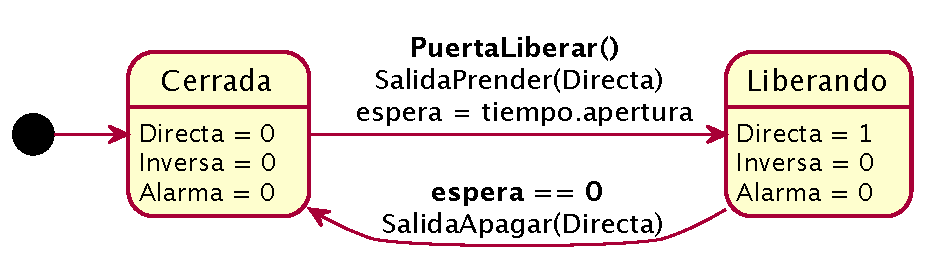
\includegraphics[width=0.9\textwidth]{Figures/PNK-DE001.pdf}
	\caption[Diagrama de estados con cerradura electromagnética y sin sensor]{Diagrama de estado para el control de una puerta sin sensor de apertura y con liberación electromagnética.}
	\label{fig:ControlSinSin}
\end{figure}

\begin{figure}[H]
	\centering
	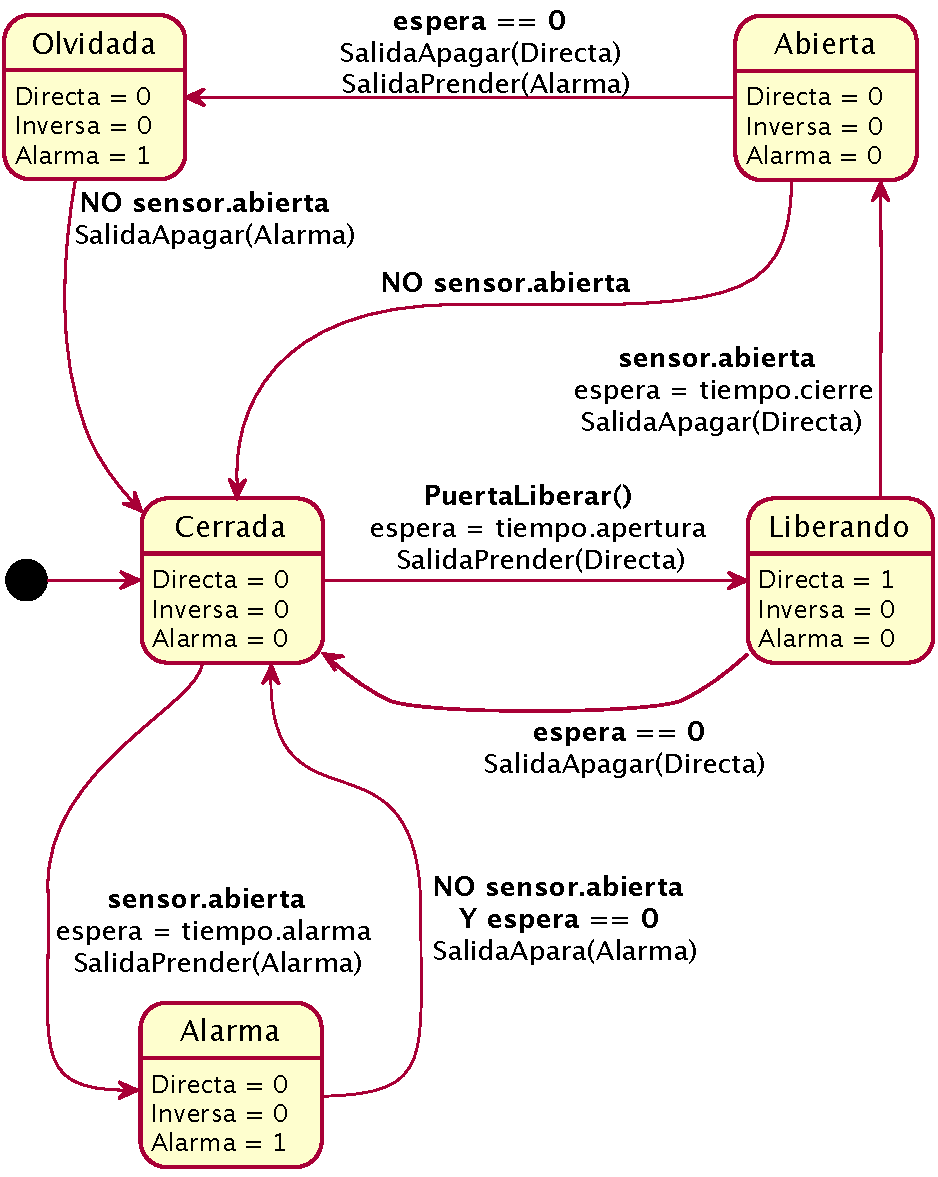
\includegraphics[width=0.9\textwidth]{Figures/PNK-DE002.pdf}
	\caption[Diagrama de estados con cerradura electromagnética y sensor]{Diagrama de estado para el control de una puerta con sensor de apertura y con liberación electromagnética.}
	\label{fig:ControlSinCon}
\end{figure}

\begin{figure}[H]
	\centering
	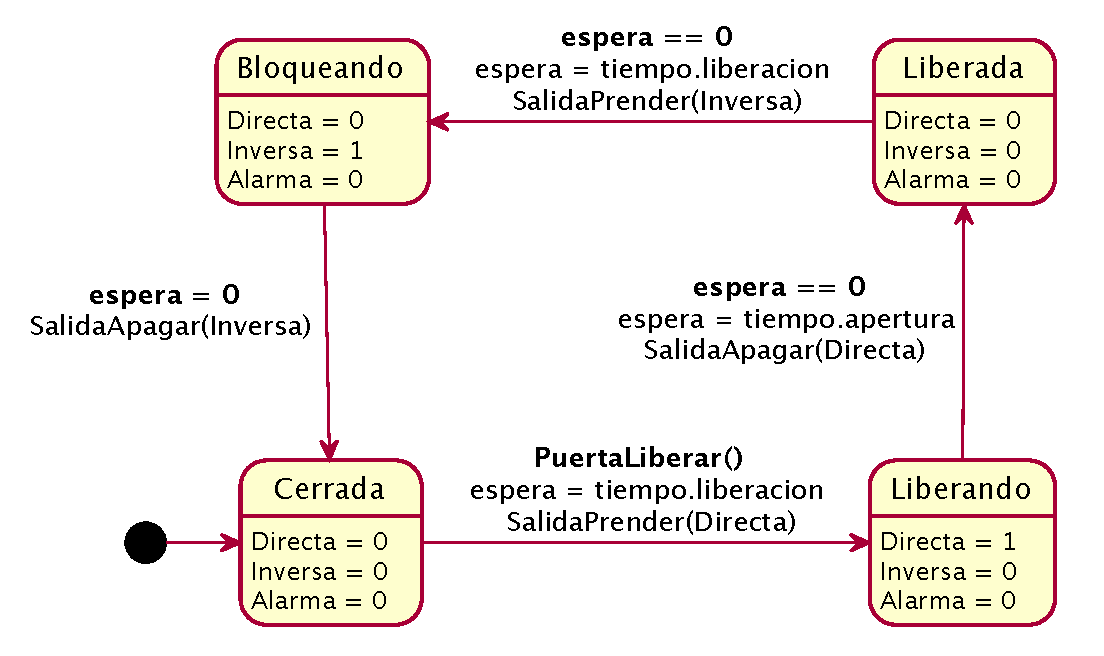
\includegraphics[width=0.9\textwidth]{Figures/PNK-DE003.pdf}
	
	\caption[Diagrama de estados con cerradura motorizada y sin sensor]{Diagrama de estado para el control de una puerta sin sensor de apertura y con liberación motorizada.}
	\label{fig:ControlConSin}
\end{figure}

\begin{figure}[ht]
	\centering
	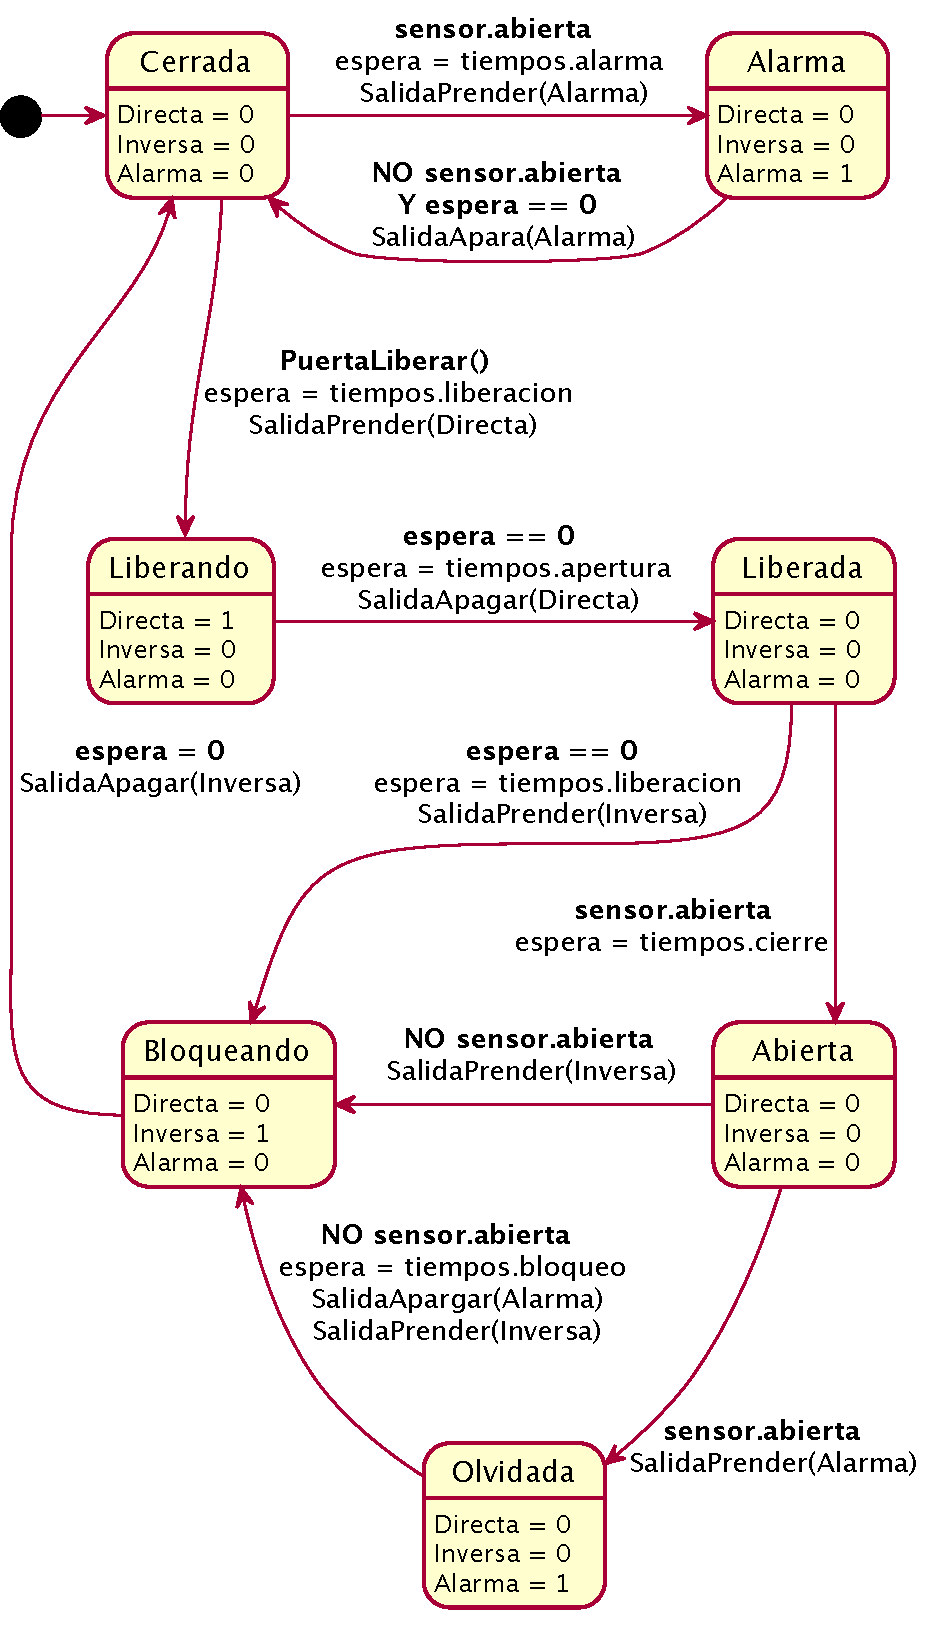
\includegraphics[width=0.9\textwidth]{Figures/PNK-DE004.pdf}
	\caption[Diagrama de estados con cerradura motorizada y sensor]{Diagrama de estado para el control de una puerta con sensor de apertura y con liberación motorizada.}
	\label{fig:ControlConCon}
\end{figure}
	
	\item ArbolB: encapsula toda la gestión de un índice utilizando la estructura de datos denominada ArbolB  o \emph{BTree}. Permite aprovechar las transferencias de bloques en los almacenamientos secundarios, como la tarjeta microSD, para disminuir el tiempo de búsqueda y actualización de una lista ordenada. Tanto la clase Editor, que se explica a continuación, como esta son también componentes críticos del sistema, ya que cualquier error en ellas se traduce en que personas autorizadas no puedan ingresar, o peor aún, en accesos de personas no autorizadas. Pero a diferencia de la clase Puertas, en estas el aspecto crítico está en la implementación y no en el diseño, ya que los algoritmos que se utilizan son ampliamente conocidos.
		
	\item Editor: encapsula toda la gestión de una actualización que involucra múltiples escrituras en un archivo. Permite asegurar que el contenido del índice de tarjetas autorizadas no resultará corrupto por una modificación incompleta. Esta clase utiliza el concepto de transacción ACID (\emph{Atomicity, Consistency, Isolation and Durability)} muy común en las bases de datos relacionales, que en nuestro caso se puede resumir en que cualquier cambio al índice se realiza siempre de manera completa, o de lo contrario, no efectúa absolutamente ningún cambio. Para la implementación se utilizó un archivo de transacciones donde se registran las escrituras de los sectores que se van actualizando en el índice. Al completar la modificación, esta se confirma en el mismo archivo de transacciones, y a partir de este punto se comienzan a aplicar los cambios en el archivo de datos. Si ocurre una interrupción del proceso, por ejemplo por un reinicio del sistema, primero se buscan transacciones confirmadas para aplicar los cambios nuevamente y recién entonces se comienza la operación del sistema.

\FloatBarrier

	\item Autorizados: encapsula toda la gestión de una lista con las tarjetas autorizadas a ingresar. Permite consultar si una tarjeta está autorizada, recuperar toda la lista de tarjetas autorizadas y agregar o eliminar una tarjeta en ella. Esta clase agrega muy poca lógica y es prácticamente un adaptador de la clase ArbolB para convertir la funcionalidad de un índice en una lista presente/ausente. Esta clase agrega además el control de sección crítica necesario para que el índice pueda ser consultado y actualizado por dos tareas diferentes que se ejecutan en forma concurrente.

	\item Sensores: encapsula toda la gestión de filtro digital asociado a terminales digitales de entrada. Permite definir un valor de histéresis para eliminar los eventos generados por ruido electromagnético. También permite generar eventos por cambios en el estado del sensor y determinar si la entrada digital presenta un estado estable o se encuentra en transición.

	\item Configuración: encapsula toda la gestión de las opciones de configuración del equipo. Permite consolidar las opciones que pueden cambiar en cada uno de los componentes en una estructura binaria, que puede ser convertida desde y hacia una cadena de caracteres utilizando la codificación JSON.
\end{itemize}


\subsection{Tareas del sistema}

En esta capa se encuentran las clases que implementan directamente la lógica de funcionamiento del equipo con el  mayor nivel de abstracción. Esto permite extender la funcionalidad en forma simple, dado que el código aplica, casi directamente, las reglas de negocio del equipo. Todas las clases de esta capa encapsulan tareas del sistema operativo de tiempo real que se ejecutan en forma concurrente. Las clases que componen esta capa son:

\begin{itemize}
	\item Sonidos: encapsula toda la reproducción de una melodía monofónica en un parlante. Define una secuencia de notas especificando la frecuencia y duración de las mismas, y de esta manera permite generar dos sonidos distintivos para diferenciar los accesos autorizados de los rechazados.
	
	\item Lectora: encapsula toda la comunicación con la lectora y, por medio de esta, con la tarjeta de proximidad. Permite recuperar el número de serie único asignado a la tarjeta y genera un evento al control para informar de una nueva lectura.

	\item Control: encapsula toda la gestión de las reglas para la apertura y supervisión de la puerta. Esta clase implementa un patrón de diseño de software denominado control ambiental. De esta forma convergen en un solo punto los eventos de la clase Puerta, de la clase Sensor, de la clase Lectora y de la clase Autorizados para centralizar la respuesta y el registro a estos eventos. 
	
	\item Bitacora: encapsula el proceso de registro en un archivo de los eventos generados por el control. Permite efectuar la escritura en el archivo, una operación lenta, en forma diferida para minimizar la interferencia en los tiempos de operación del control de la puerta.
	
	\item Servidor: encapsula todo el servicio de comunicación para la gestión del equipo. Permite configurar la interfaz WiFi, iniciar un servidor HTTP y atender los pedidos recibidos interactuando con las clases Reloj, Bitacora, Configuracion y Autorizados para completar las operaciones solicitadas.
	
\end{itemize}

De la descripción anterior se desprende que la correcta interacción entre las clases de esta capa resulta clave para lograr el funcionamiento esperado del equipo. La ingeniería de software nos brinda una herramienta para poder representar estas interacciones entre los componentes de un programa: los diagramas de secuencia UML. En estos se representan las llamadas a métodos de las diferentes clases siguiendo los casos de uso analizados en la subsección \ref{sub:CasosDeUso}. Los diagramas más importantes pueden verse en las figuras \ref{fig:SecuanciaPulsador}, \ref{fig:SecuenciaTarjeta}, \ref{fig:SecuenciaForzada} y \ref{fig:SecuenciaConfiguracion}.

\begin{figure}[ht]
	\centering
	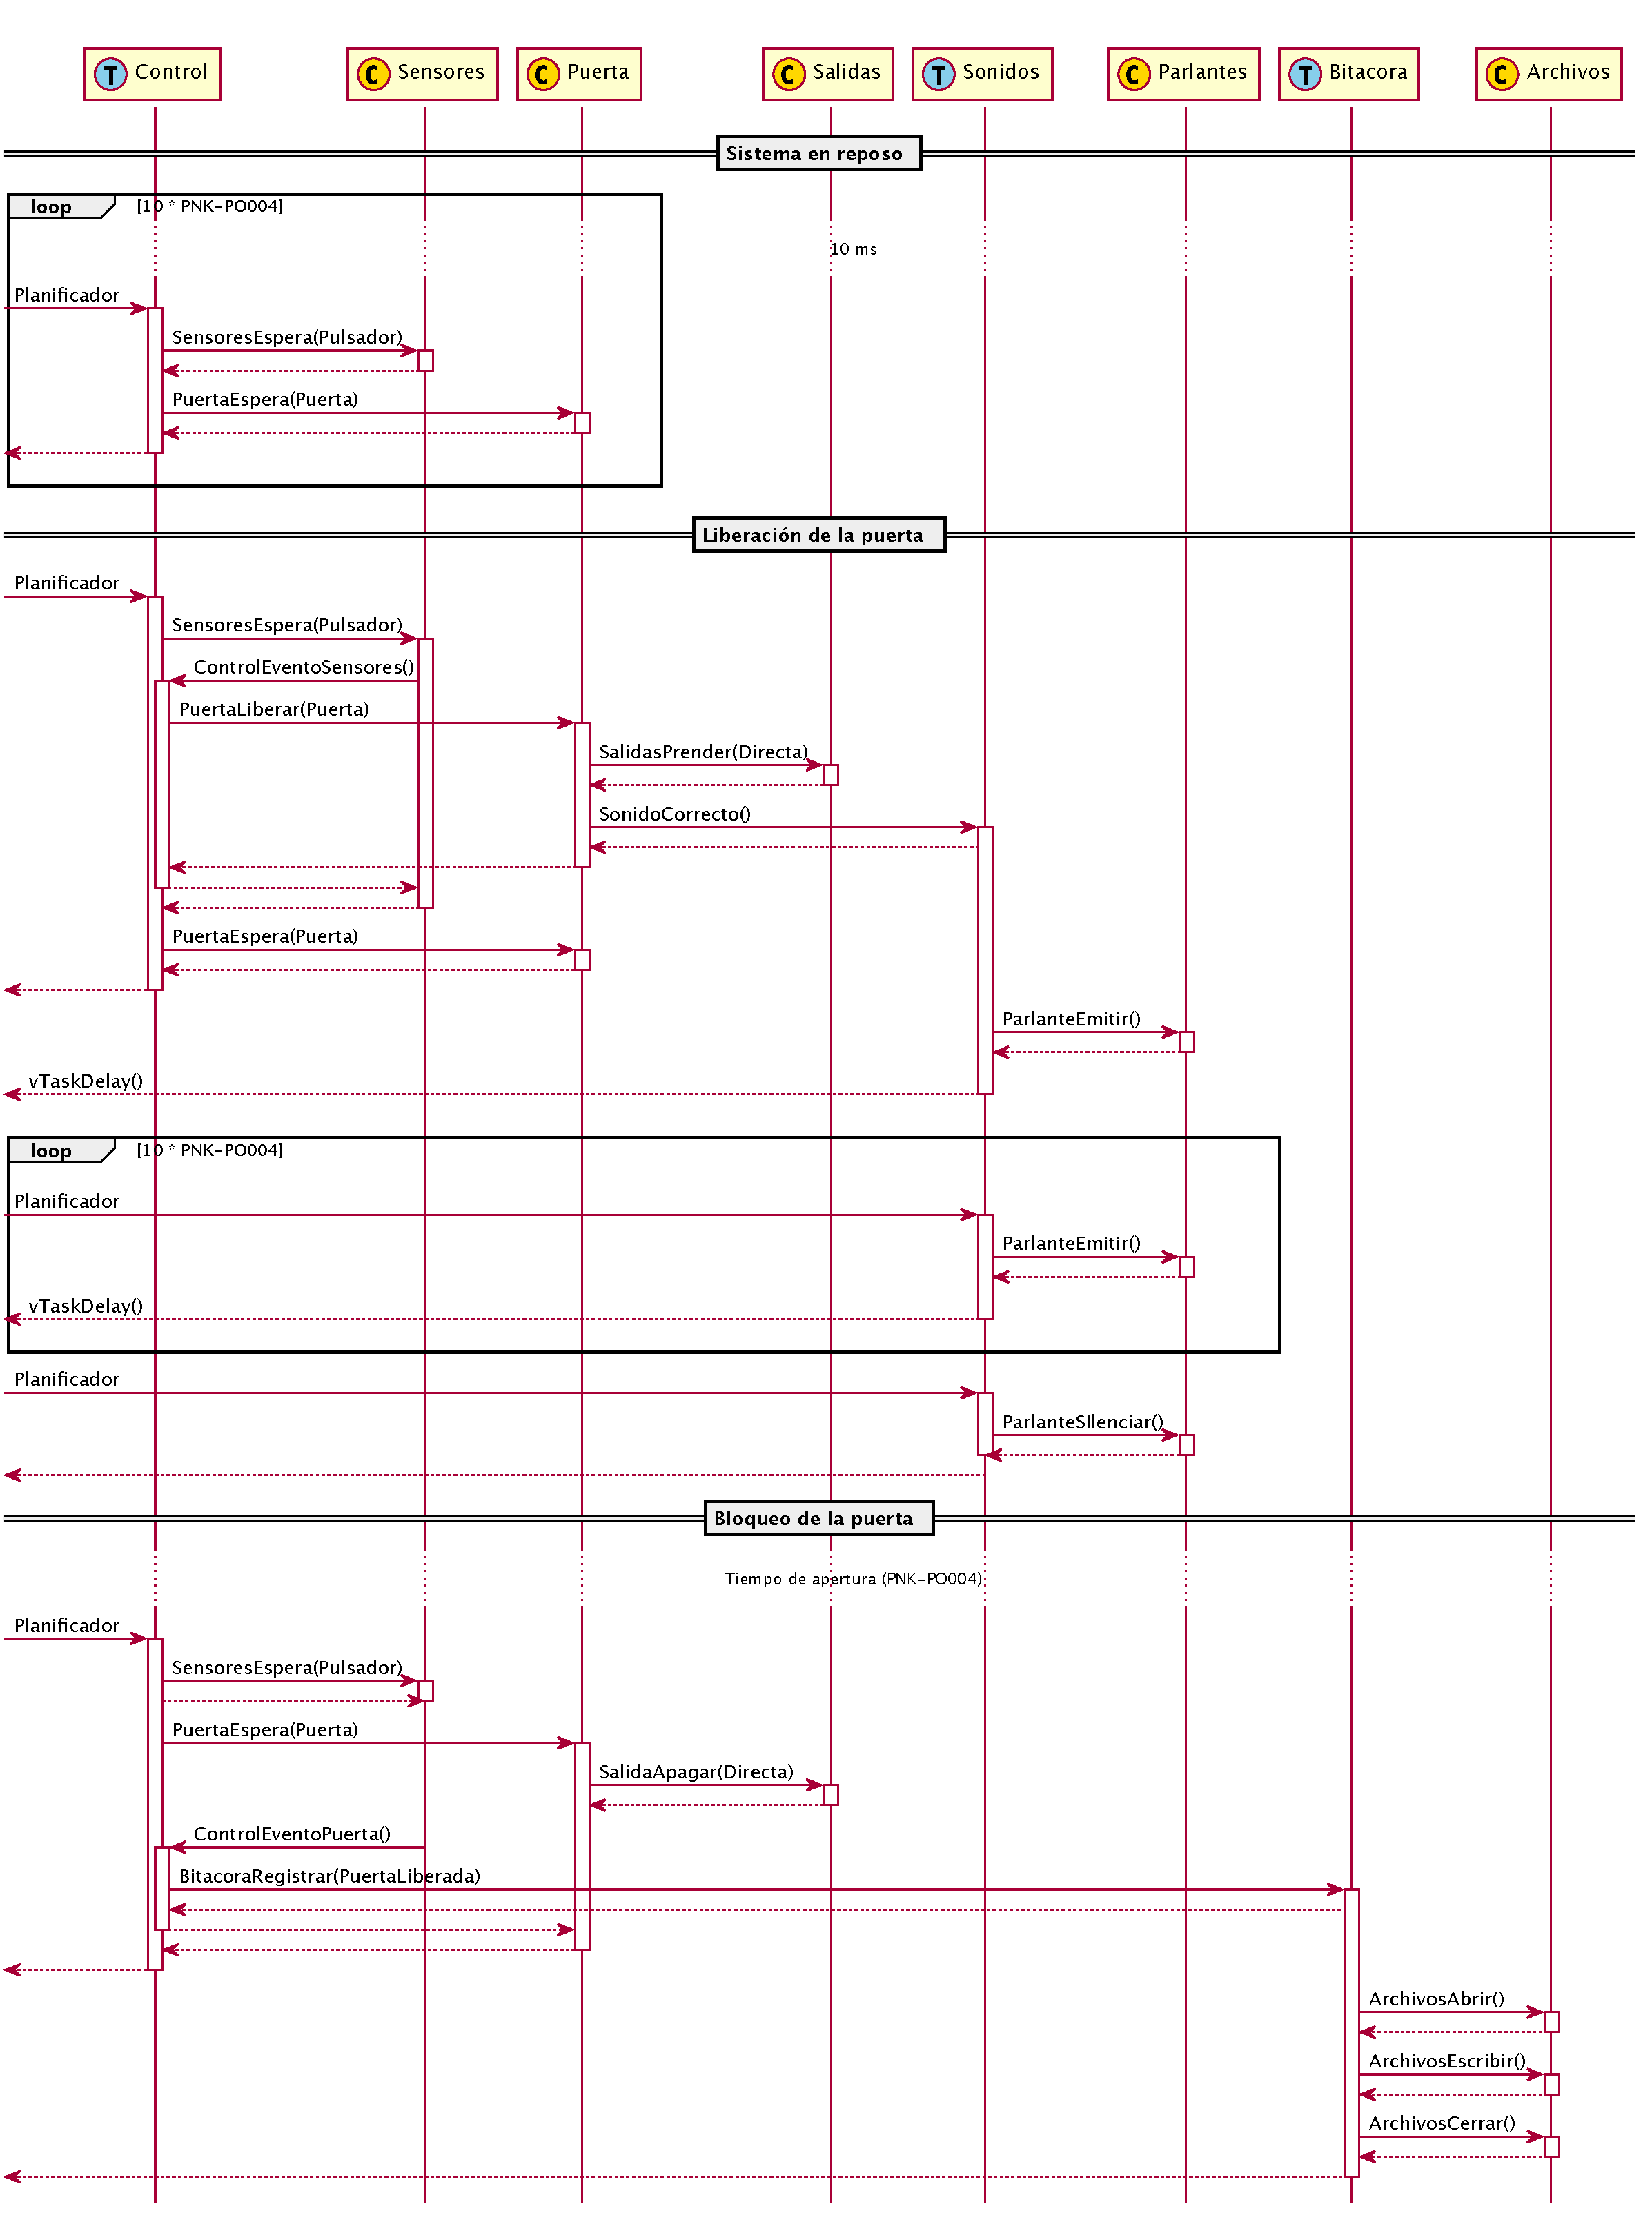
\includegraphics[width=\textwidth]{Figures/PNK-DS001.pdf}
	\caption[Apertura por pulsador con cerradura electromagnética y sin sensor]{Diagrama de secuencia para la liberación por pulsador de una puerta, sin sensor de apertura y con liberación electromagnética.}
	\label{fig:SecuanciaPulsador}
\end{figure}

\begin{figure}[ht]
	\centering
	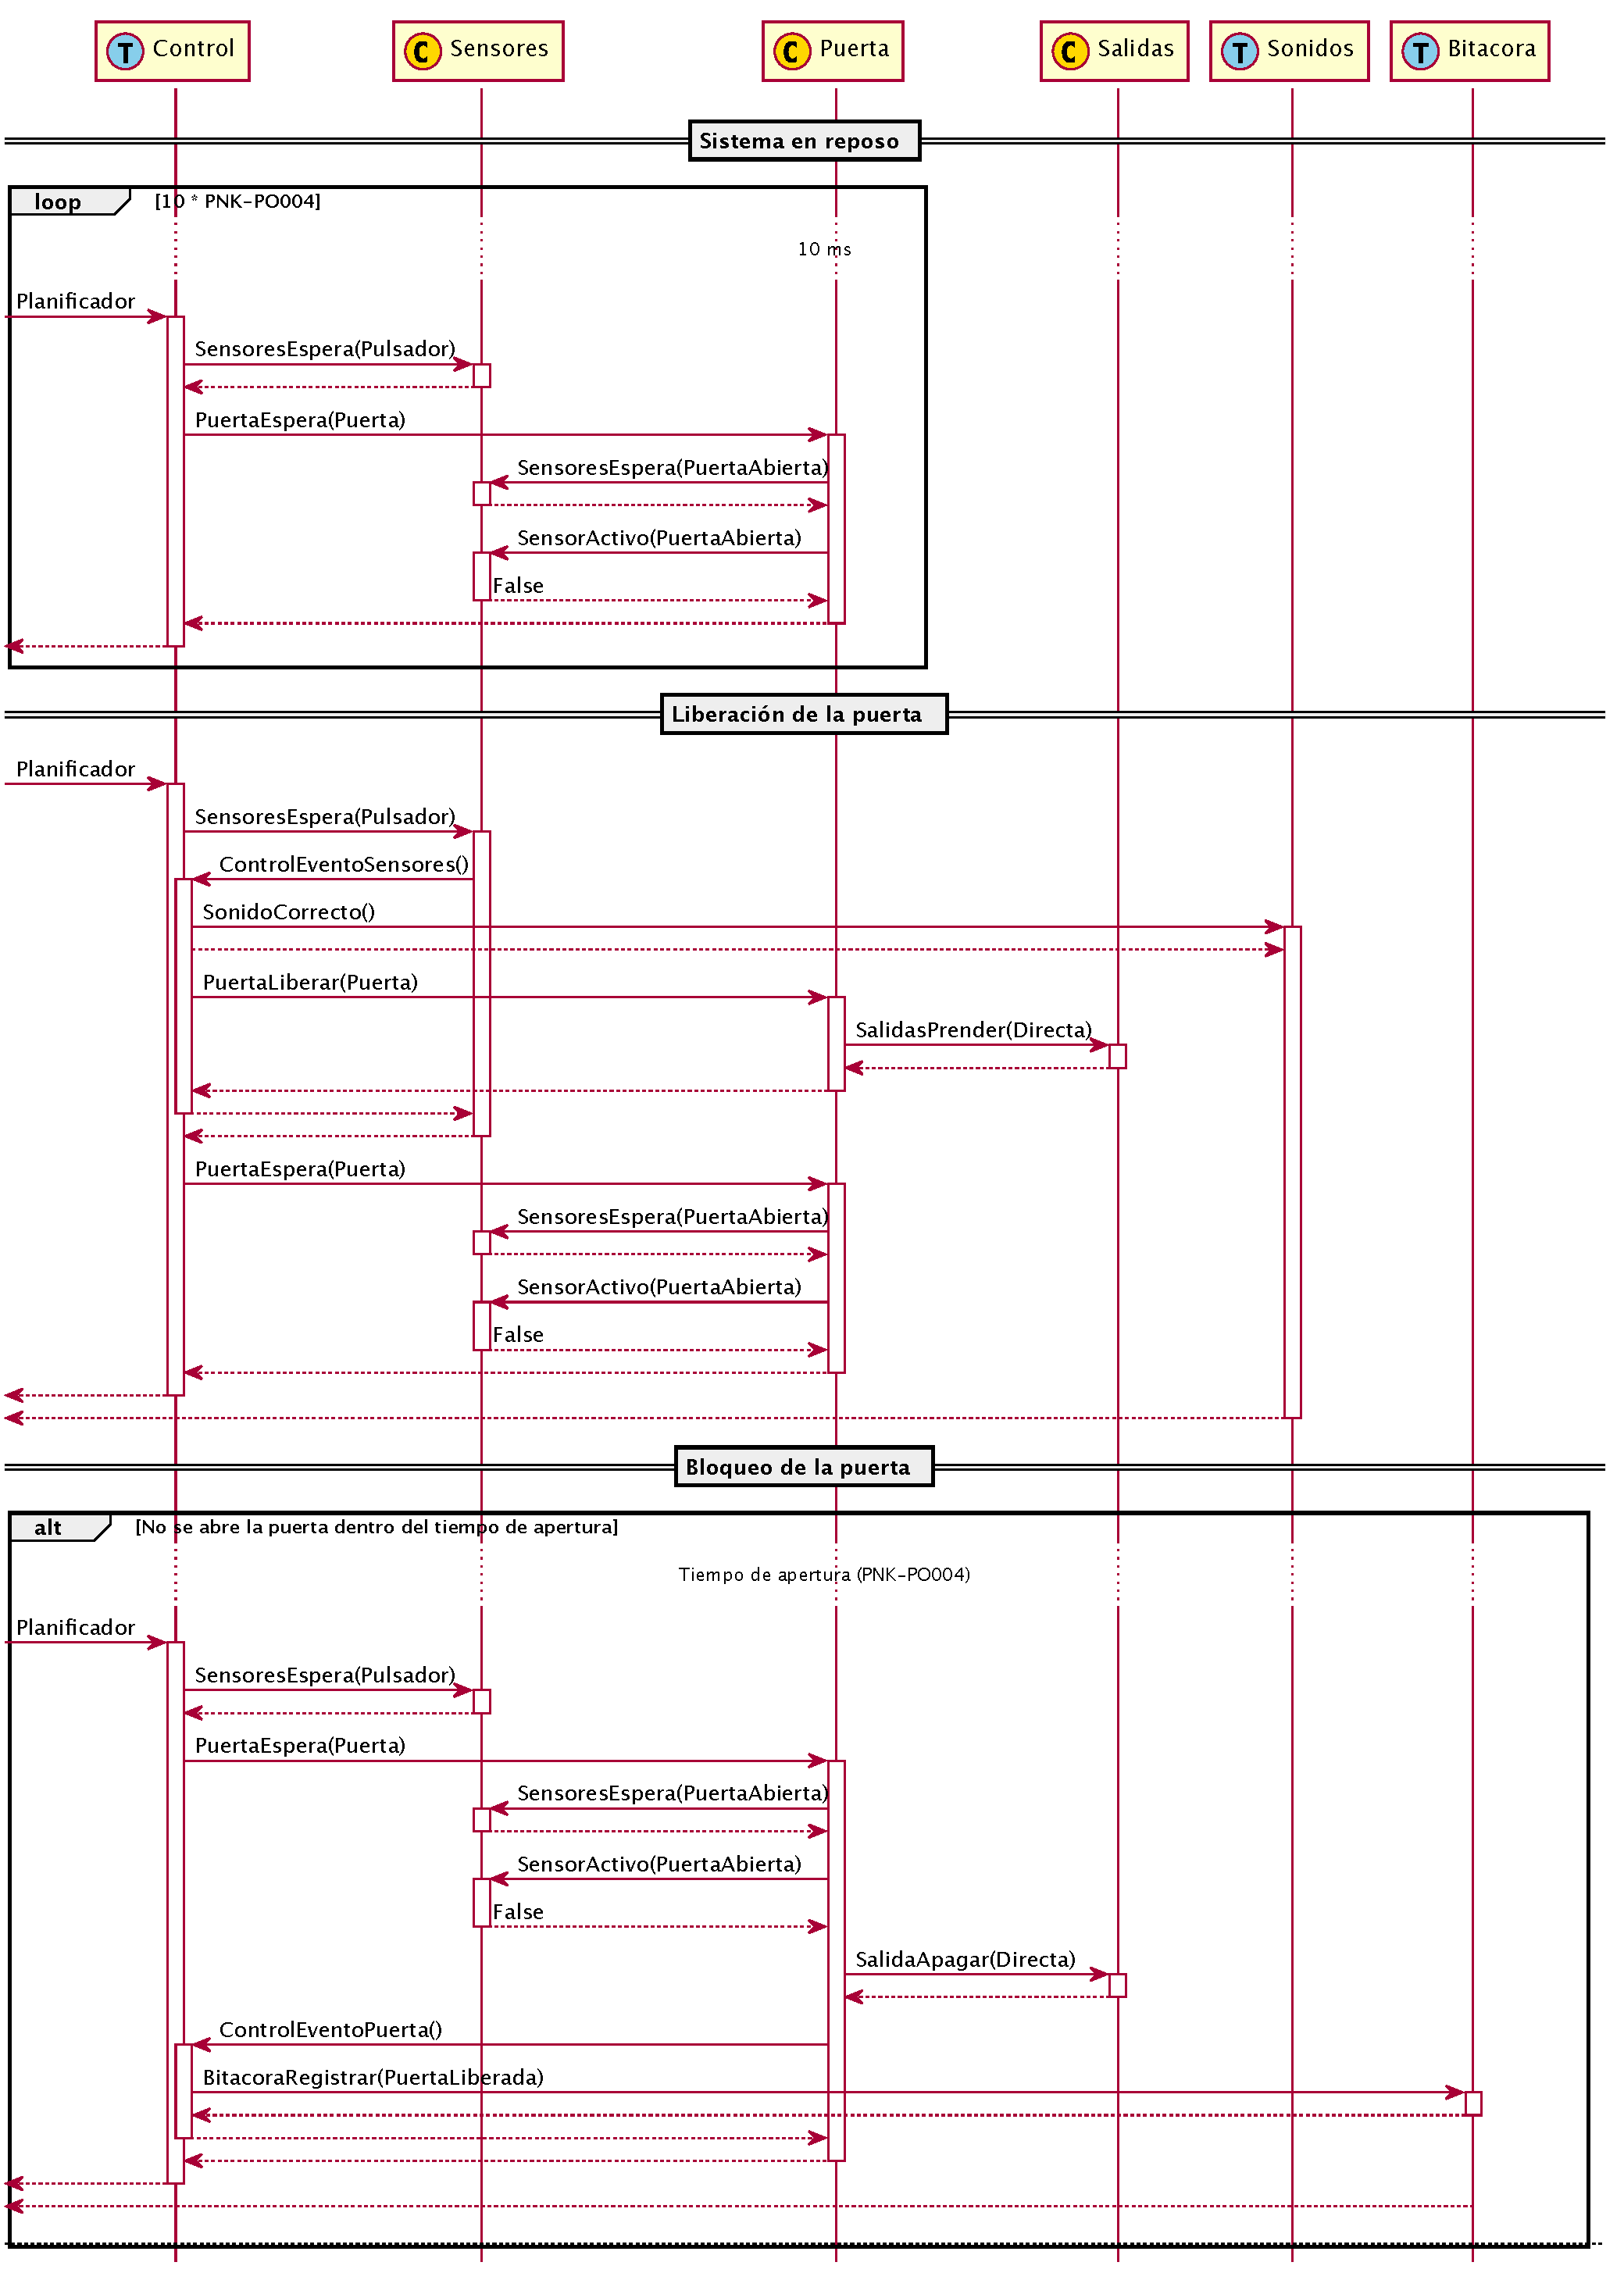
\includegraphics[width=\textwidth]{Figures/PNK-DS002-A.pdf}
	{\color{red} No es el diagrama correcto pero tiene la misma forma y extensión}
	\caption[Apertura por tarjeta con cerradura electromagnética y sensor]{Diagrama de secuencia para la apertura y cierre por tarjeta de proximidad, con sensor de apertura y con liberación electromagnética.}
	\label{fig:SecuenciaTarjeta}
\end{figure}

\begin{figure}[ht]
	\centering
	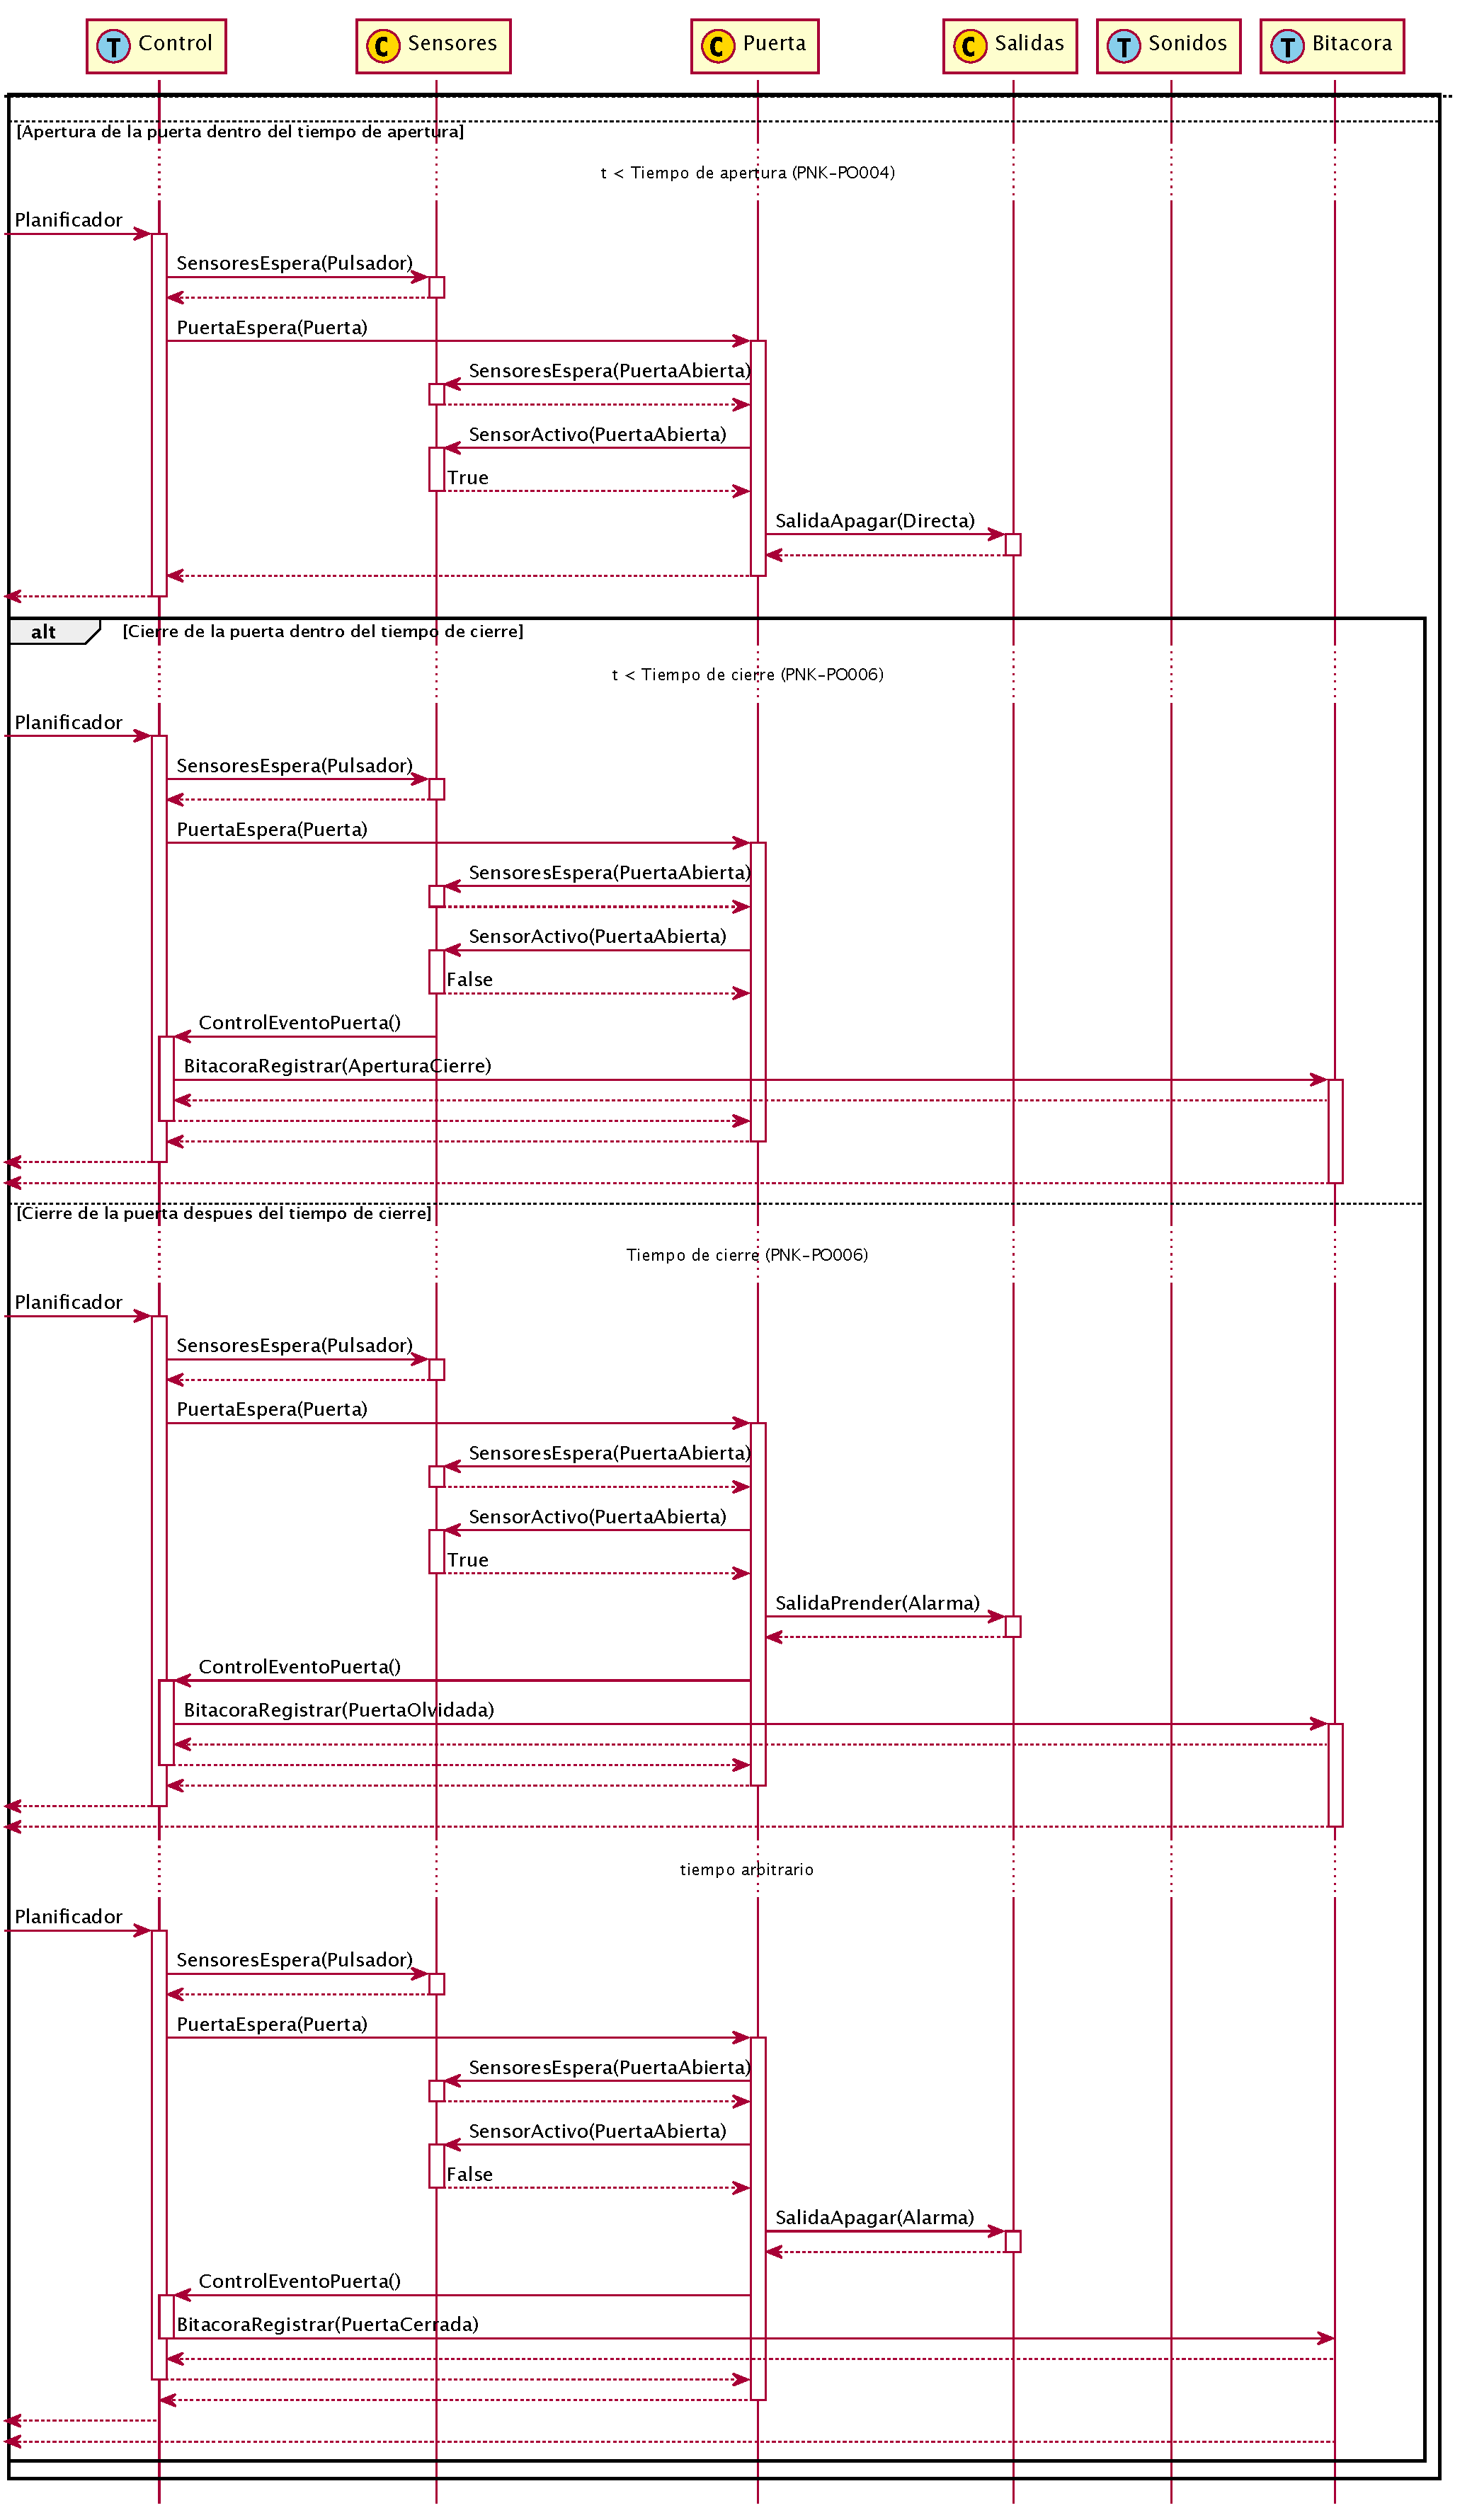
\includegraphics[width=\textwidth]{Figures/PNK-DS002-B.pdf}
	{\color{red} No es el diagrama correcto pero tiene la misma forma y extensión}
	\caption[Alarma por apertura forzada de la puerta]{Diagrama de secuencia para la activación de alarma por apertura forzada de la puerta.}
	\label{fig:SecuenciaForzada}
\end{figure}

\begin{figure}[ht]
	\centering
	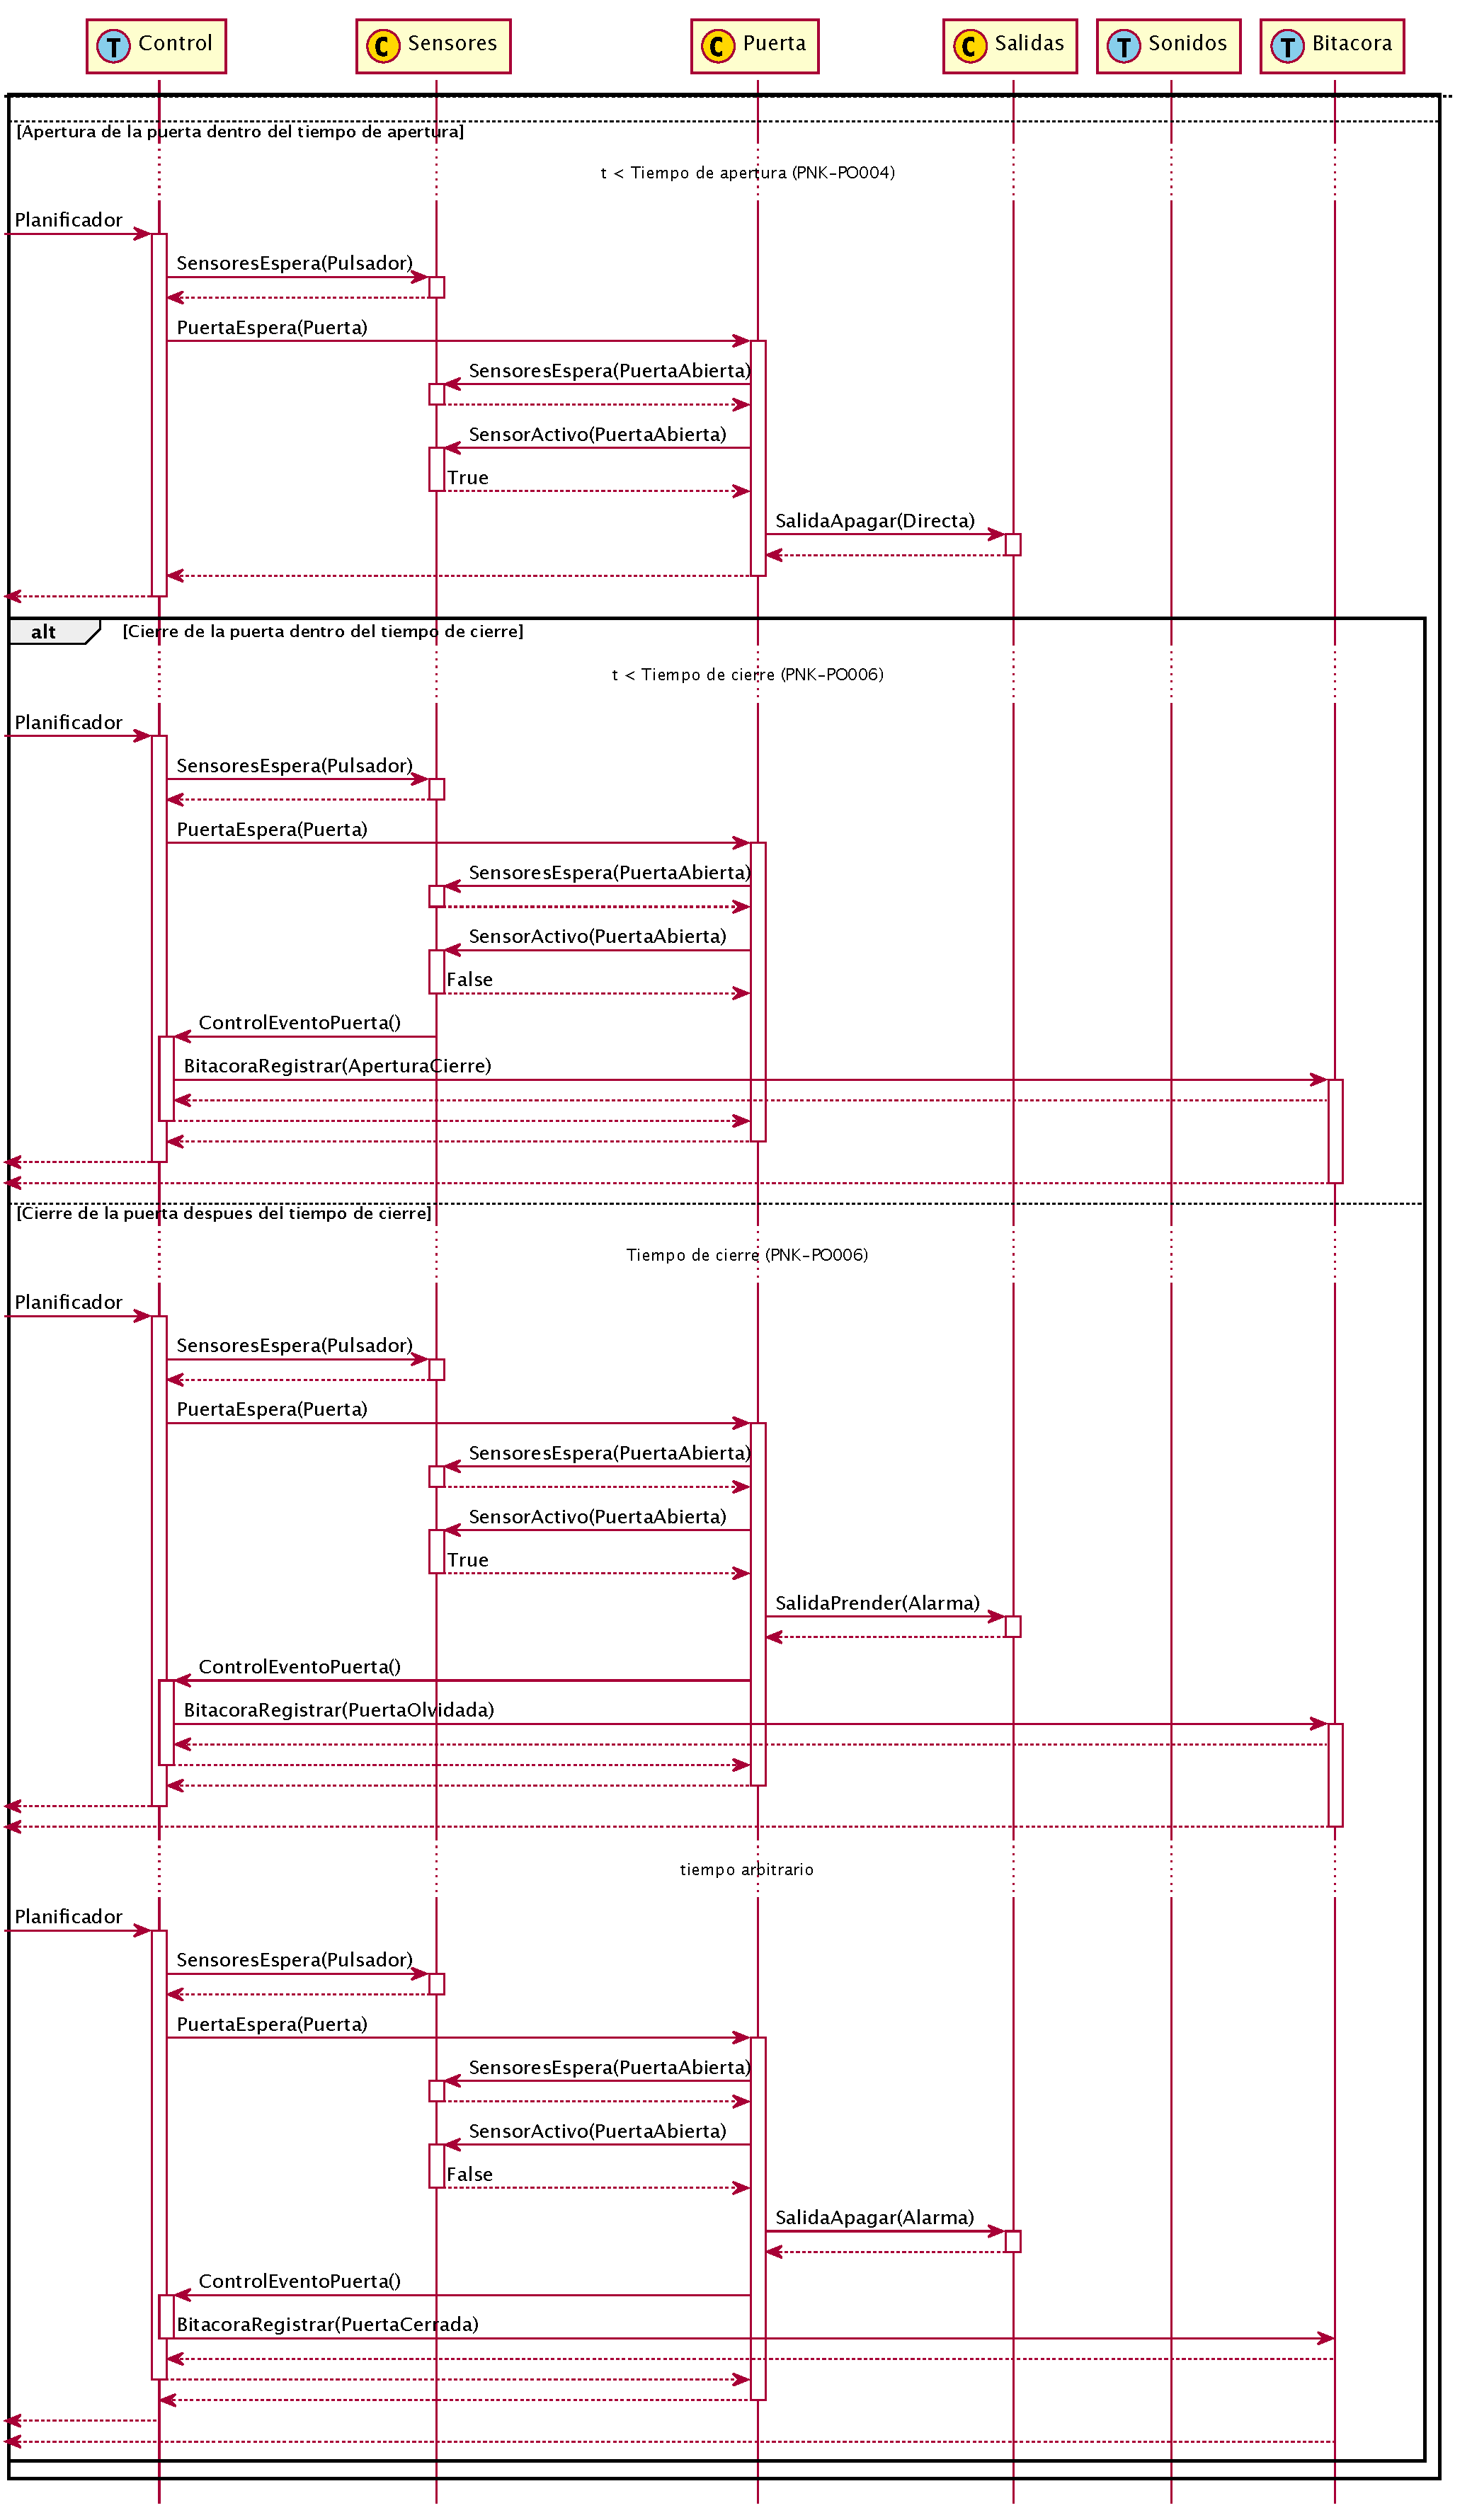
\includegraphics[width=\textwidth]{Figures/PNK-DS002-B.pdf}
	{\color{red} No es el diagrama correcto pero tiene la misma forma y extensión}
	\caption[Secuencia para el cambio de configuración]{Diagrama de secuencia para el cambio de configuración del equipo.}
	\label{fig:SecuenciaConfiguracion}
\end{figure}

\FloatBarrier

\section{Desarrollo del firmware}
\label{sec:desarrollo}

\subsection{Entorno de desarrollo}

Las metodologías de desarrollo propuestas por la ingeniería de software son lineamientos generales que deben ser ajustados a la realidad del equipo de desarrollo, y un proyecto que se inicia desde cero siempre es una buena oportunidad para adoptar nuevas metodologías. Por esta razón se decidió aplicar TDD (\emph{Test Driven Development}) para todo el proceso de codificación. Esta estrategia de trabajo plantea el desarrollo de una prueba unitaria que valida un requerimiento específico en primer lugar, y recién después el código de producción necesario para la implementación. Pero es un requisito indispensable disponer de una herramienta que compile y ejecute las pruebas unitarias en forma automática para poder implementar esta propuesta. La herramienta seleccionada para esta tarea fue Ceedling, un desarrollo en Ruby de código abierto pensado para implementar TDD en sistemas embebidos. Aunque realmente está formada por tres componentes que pueden ser utilizados en forma independiente, estos se acoplan perfectamente para funcionar como una solución integral. A estos se pueden sumar \emph{plugins}, propios o de terceros, que permiten agregar nuevas funcionalidades. Las componentes utilizadas en este trabajo fueron:

\begin{itemize}
	\item Unity: provee una variedad de funciones para verificar los resultados esperados en las pruebas unitarias. Estas funciones pueden comparar diferentes tipos de datos, e informan las discrepancias cuando los valores no son los correctos.

	\item Fake Function Framework: provee la capacidad de generar funciones Mock o Stub que permiten reemplazar las dependencias para poder implementar pruebas unitarias en clases que requieren código que no se desea probar.
	
	\item Ceedling: provee la compilación, ejecución y consolidación de los resultados de las pruebas unitarias, en forma automática y con un mínimo esfuerzo de configuración.
	
	\item GCOV: provee métricas con la cobertura de las pruebas ejecutadas, es decir la proporción de líneas de código fuente o de condiciones lógicas que fueron verificadas al ejecutar las pruebas unitarias.
	
	\item CLOC: provee métricas con la cantidad de comentarios y líneas de código fuente, para generar estadísticas que determinen la calidad del código.  
\end{itemize}

Otro de los aspectos que se buscó optimizar desde el inicio del proyecto fue la documentación, tanto del diseño general como del código en sí mismo. Para esto se seleccionaron dos herramientas también de código abierto que tienen la capacidad de trabajar en conjunto como si fueran una sola. Para la documentación del código se utilizó Doxygen, una programa que tiene la capacidad de generar la documentación de una biblioteca a partir de comentarios especiales ubicados en el código fuente. Para la escritura de los documentos de diseño se decidió utilizar la sintaxis Markdown y procesarlos también con Doxygen para unificar en un solo sitio WEB toda la información del desarrollo. Para los diagramas UML se utilizó PlantUML, una herramienta también de código abierto que puede funcionar en conjunto con Doxygen, y que permite generar los diagramas a partir de descripciones textuales muy simples y rápidas.

Finalmente, como entorno de desarrollo integrado se decidió utilizar Visual Studio Code, un editor de código abierto desarrollado por Microsoft, que funciona en las plataformas de Windows, Linux y MacOS indistintamente. Tiene además una extensa biblioteca de \emph{plugins} que le permiten extender la funcionalidad básica. De esta forma fue posible agregarle el reconocimiento de la sintaxis en el lenguaje C en los comentarios Doxygen, en los documentos Markdown y en los diagramas PlantUML. También se pudo disponer del procesamiento las advertencias por errores en la documentación devueltos por Doxygen, de la visualización de los diagramas UML generados por PlantUML, de la ejecución de las pruebas unitarias mediente Ceedling y de la gestión del repositorio GIT que almacenó el código. A estas herramientas debemos agregarles el ESP-IDF (\emph{Espressif IoT Development Framework}), el conjunto de bibliotecas y utilidades provistas por el fabricante del procesador para el desarrollo del software para los procesadores ESP32. De esta forma queda completo el entorno de desarrollo utilizado para el presente trabajo. En la tabla \ref{tab:HerramientasDesarrollo} se puede ver un resumen con el nombre de cada herramienta y una breve descripción de la función.

\begin{table}[ht]
	\centering
	\caption[Herramientas utilizadas para el desarrollo del firmware]{Resumen de herramientas utilizadas en el desarrollo del firmware del presente trabajo.}
	\begin{tabular}{L{25mm} L{100mm}}    
		\toprule
		\textbf{Nombre} & 
		\textbf{Funcionalidad proporcionada} \\
		\midrule
		Unity & 
		Verificación de los resultados en las pruebas unitarias y reporte de las discrepancias \\
		Fake Function Framework &
		Generación automática de funciones Mock y Stub para resolver las dependencias en las pruebas unitarias \\
		Ceedling &
		Resolución automáticamente de dependencias, compilación, ejecución y consolidación los resultados de las pruebas unitarias \\
		GCOV &
		Determinación de la cobertura en las pruebas unitarias y generación de un reporte en forma de página WEB \\
		CLOC &
		Generación de estadísticas con la proporción de comentarios y pruebas por línea de código fuente \\
		Doxygen &
		Generación de la documentación consolidada con la información del diseño y del código en forma de una página WEB \\
		PlantUML &
		Generación los diagramas UML a partir de descripciones textuales \\
		GIT &
		Mantenimiento de las versiones del código fuente del firmware, de la documentación de diseño y de los diagramas UML \\
		ESP-IDF &
		Biblioteca con los controladores y las herramientas de desarrollo provistas por el fabricante de la plataforma \\
		Visual Studio Code &
		Entorno de desarrollo integrado para la edición el código fuente y el manejo centralizado de las herramientas utilizadas en el proyecto \\
		\bottomrule
		\hline
	\end{tabular}
	\label{tab:HerramientasDesarrollo}
\end{table}

\subsection{Pruebas de integración en las tareas del sistema}

La plataforma de desarrollo provista por el fabricante utiliza a FreeRTOS como sistema operativo de tiempo real, donde se ejecutan como tareas los servicios de comunicaciones como el protocolo TCP/IP y el servidor HTTP. Esta versión de FreeRTOS ha sido modificada por el fabricante para poder ejecutarse en un procesador de doble núcleo como es ESP32. Por estas razones, utilizar otro sistema operativo de tiempo real implicaría un esfuerzo de desarrollo muy importante, que excedería ampliamente los alcances del presente trabajo. 

Lamentablemente FreeRTOS es un desarrollo complejo, que además de estar modularizado para facilitar la portación a diferentes arquitecturas, tiene un código que puede personalizarse utilizando el archivo FreeRTOSConfig.h. Todo esto hacen que sea imposible generar automáticamente funciones Stub o Mock que permitan implementar pruebas unitarias automatizadas en código que utiliza los servicios del sistema operativo. 

Una de las primeras estrategias para poder conciliar la idea de aplicar TDD con los problemas derivados de utilizar FreeRTOS fue dividir la aplicación en tres capas. De esta forma se buscó concentrar el código critico en los objetos de la capa de controladores, y como estos no utilizan los servicios del sistema operativo se pudieron desarrollar utilizando TDD. De todas formas esta solución no resultó totalmente satisfactoria, por lo que se siguió buscando una alternativa para poder ejecutar pruebas automatizadas sobre las tareas.

La solución definitiva a este problema se obtuvo combinando la portabilidad de FreeRTOS y la capacidad de Ceedling de utilizar \emph{plugins}. Para esto se desarrolló un \emph{plugin} propio que analiza el código fuente del archivo de prueba para determinar si utiliza los servicios del sistema operativo. En este caso modifica el proceso de compilación y enlazado para incluir una versión FreeRTOS que ejecuta como una tarea dentro de un ambiente POSIX. También modifica el código generado para el \emph{runner} de la prueba para iniciar el sistema operativo, y mueve la secuencia de pruebas a una tarea de FreeRTOS que detiene el planificador como ultima operación.

De esta forma, Ceedling puede generar un ejecutable que inicia el sistema operativo, ejecuta cada una de las pruebas en forma secuencial y termina una vez que se completaron las pruebas. Este comportamiento, que resulta natural en las pruebas automatizadas, es totalmente contrapuesto al uso normal de FreeRTOS, donde el sistema se inicia pero nunca se detiene. El resultado final de este desarrollo es la posibilidad de implementar pruebas automatizadas sobre las tareas de la capa de aplicación con las mismas herramientas utilizadas para el resto del desarrollo.

\subsection{Uso del tipo de abstracto de datos}

Como ya se mencionó en la subsección \ref{sub:Arquitectura}, para el modelado del firmware se utilizó una metodología orientada a objetos. Uno de los inconvenientes de aplicar esta propuesta es que el lenguaje C, el más utilizado en el desarrollo de sistemas embebidos, no es un lenguaje orientado a objetos.

Para resolver este problema existe una propuesta denominada ADT (\emph{Abstract Data Type}) que, explotando el uso de punteros a estructuras, permite emular muy fácilmente una programación orientada a objetos, utilizando el lenguaje C estándar. Esta técnica considera un archivo de cabeceras (.h) como la interfaz pública de la clase y el archivo de código fuente (.c) como la implementación privada, y  plantea el siguiente patrón de programación:

\begin{enumerate}
	\item La declaración incompleta de una estructura de datos en el archivo de cabeceras, que define el nombre pero sin enumerar los miembros. La declaración de esta estructura se realiza en forma completa en el archivo de código, y cada uno de sus campos es equivalente a un atributo privado del objeto.
	
	\item La declaración de un puntero a esta estructura también en el archivo de cabeceras. Este tipo de puntero podrá ser utilizado desde cualquier parte del proyecto, siempre que no se intente acceder al contenido de memoria referenciado. Esto permite encapsular los atributos del objeto y evitar que puedan ser alterados en forma externa.
	 
	\item Una o más funciones que devuelven como resultado un puntero a la estructura declarado en el apartado anterior. Estas funciones son el equivalente a los constructores de la clase, y además son responsables de la alocación del espacio de memoria necesario para almacenar la nueva instancia del objeto. Esta alocación podrá ser dinámica, y utilizar funciones como \emph{malloc}, o estática mediante un arreglo de estructuras.
	
	\item Varias funciones que reciben como primer parámetro el puntero retornado por las funciones constructoras, y que son equivalentes a los métodos públicos de la clase. 
\end{enumerate}

Este patrón de programación permite generar un código que puede escalar muy fácilmente, ya que resulta irrelevante la cantidad de instancias de un mismo elemento. De esta forma, a pesar de que el software desarrollado solo puede controlar una puerta, puede inmediatamente funcionar con dos o más puertas con solo efectuar dos llamadas al constructor de la clase Puerta. En las siguientes fracciones de código puede verse un ejemplo simplificado del patrón de programación descrito.

\begin{lstlisting}[caption=Porción simplificada del archivo de cabecera con la interfaz publica de la clase Puerta.] 
/* === Declaraciones de tipos de datos ====================== */
//! Tipo de datos para referenciar a un objeto puerta
typedef struct puerta_s * puerta_t;

/* === Declaraciones de funciones externas ================== */
//! Función para instanciar un objeto puerta
puerta_t PuertaCrear(void);

//! Función para configurar una puerta
bool PuertaConfigurar(puerta_t puerta, tiempo_t apertura);

//! Función para liberar la puerta y permitir un ingreso
void PuertaLiberar(puerta_t puerta);
\end{lstlisting}

\begin{lstlisting}[caption=Porción simplificada del archivo de código fuente con la implementación de la clase Puerta.] 
/* === Definicion y Macros ================================== */
//! Cantidad maxima de puertas alocadas estaticamente
#define PUERTAS_CANTIDAD                1

/* === Declaraciones de tipos de datos ====================== */
//! Estructura que describe la información de una puerta
struct puerta_s {
    puerta_estado_t estado;
    tiempo_t apertura;
    tiempo_t espera;
};

/* === Definiciones de funciones internas =================== */
//! Aloca la memoria necesaria para un nuevo objeto puerta
static puerta_t CrearInstancia(void) {
    puerta_t resultado = NULL;

    static int usadas = 0;
    static struct puerta_s puertas[PUERTAS_CANTIDAD] = {0};
    
    if (usadas < sizeof(puertas) / sizeof(struct puerta_s)) {
        memset(&puertas[usadas], 0, sizeof(struct puerta_s));
        resultado = &puertas[usadas];
        usadas++;
    }
    return resultado;
}

/* === Definiciones de funciones externas =================== */
puerta_t PuertaCrear(void) {
    puerta_t self = CrearInstancia();

    if (self != NULL) {
        self->estado = PUERTA_CERRADA;
        self->espera = 0;
    }
    return self;
}

bool PuertaConfigurar(puerta_t self, tiempo_t apertura) {
    bool resultado = false;

    if (self != NULL) {
        self->apertura = apertura;
        resultado = true;
    }
    return resultado;
}

void PuertaLiberar(puerta_t self) {
    if (self != NULL) {
        if (self->estado == PUERTA_CERRADA) {
            self->espera = self->apertura - 1;
            self->estado = PUERTA_LIBERADA;
        }
    }
}

\end{lstlisting}


